\documentclass[french,12pt]{report}
\usepackage{babel}
\usepackage{a4}
%\usepackage[dvips]{graphics}
%\usepackage[pdftex]{graphicx}
\usepackage{graphicx}

\title{Projet de modelisation}
\author{Julien \textsc{Gein}
\and Jonathan \textsc{Mimouni}
\and Jean-Daniel \textsc{Michaud}}

\date{Le \today}

\begin{document}
\maketitle
\strut\thispagestyle{empty}
\vfill
\pagebreak
\setcounter{page}{1}
\tableofcontents
\pagebreak

\sloppy


\section*{Specifications}
\addcontentsline{toc}{chapter}{Specifications}
\markboth{\uppercase{Specifications}}
{\uppercase{Specifications}}

Le but principal de ce projet est de r\'ealiser un jeu de dames en java
bas\'e sur une architecture centralis\'ee (un serveur, plusieurs clients)
et une base de donn\'ees Oracle.

Le logiciel pourra enregistrer et charger l'\'etat et l'historique
d'une partie. Ce qui offriras la possibilit\'e de rejouer coup \'a coup
une partie sauvegard\'ee. Le logiciel sera aussi capable de calculer
l'ELO d'un joueur, de centraliser plusieurs parties et de permettre
a des utilisateurs distants de suivre les parties sans \^etre joueur.

Les r\`egles du jeu de dames peuvent \^etre modifi\'ees \'a la guise de
l'utilisateur. Augmenter le nombre de joueurs par partie, modifications du 
plateau de jeu, modifications des cases speciales, etc ...


\pagebreak

\section*{Diagramme de cas d'utilisation}
\addcontentsline{toc}{chapter}{Diagramme de cas d'utilisation}
\markboth{\uppercase{Diagramme de cas d'utilisation}}
{\uppercase{Diagramme de cas d'utilisation}}

\begin{center}

\begin{figure}[h]
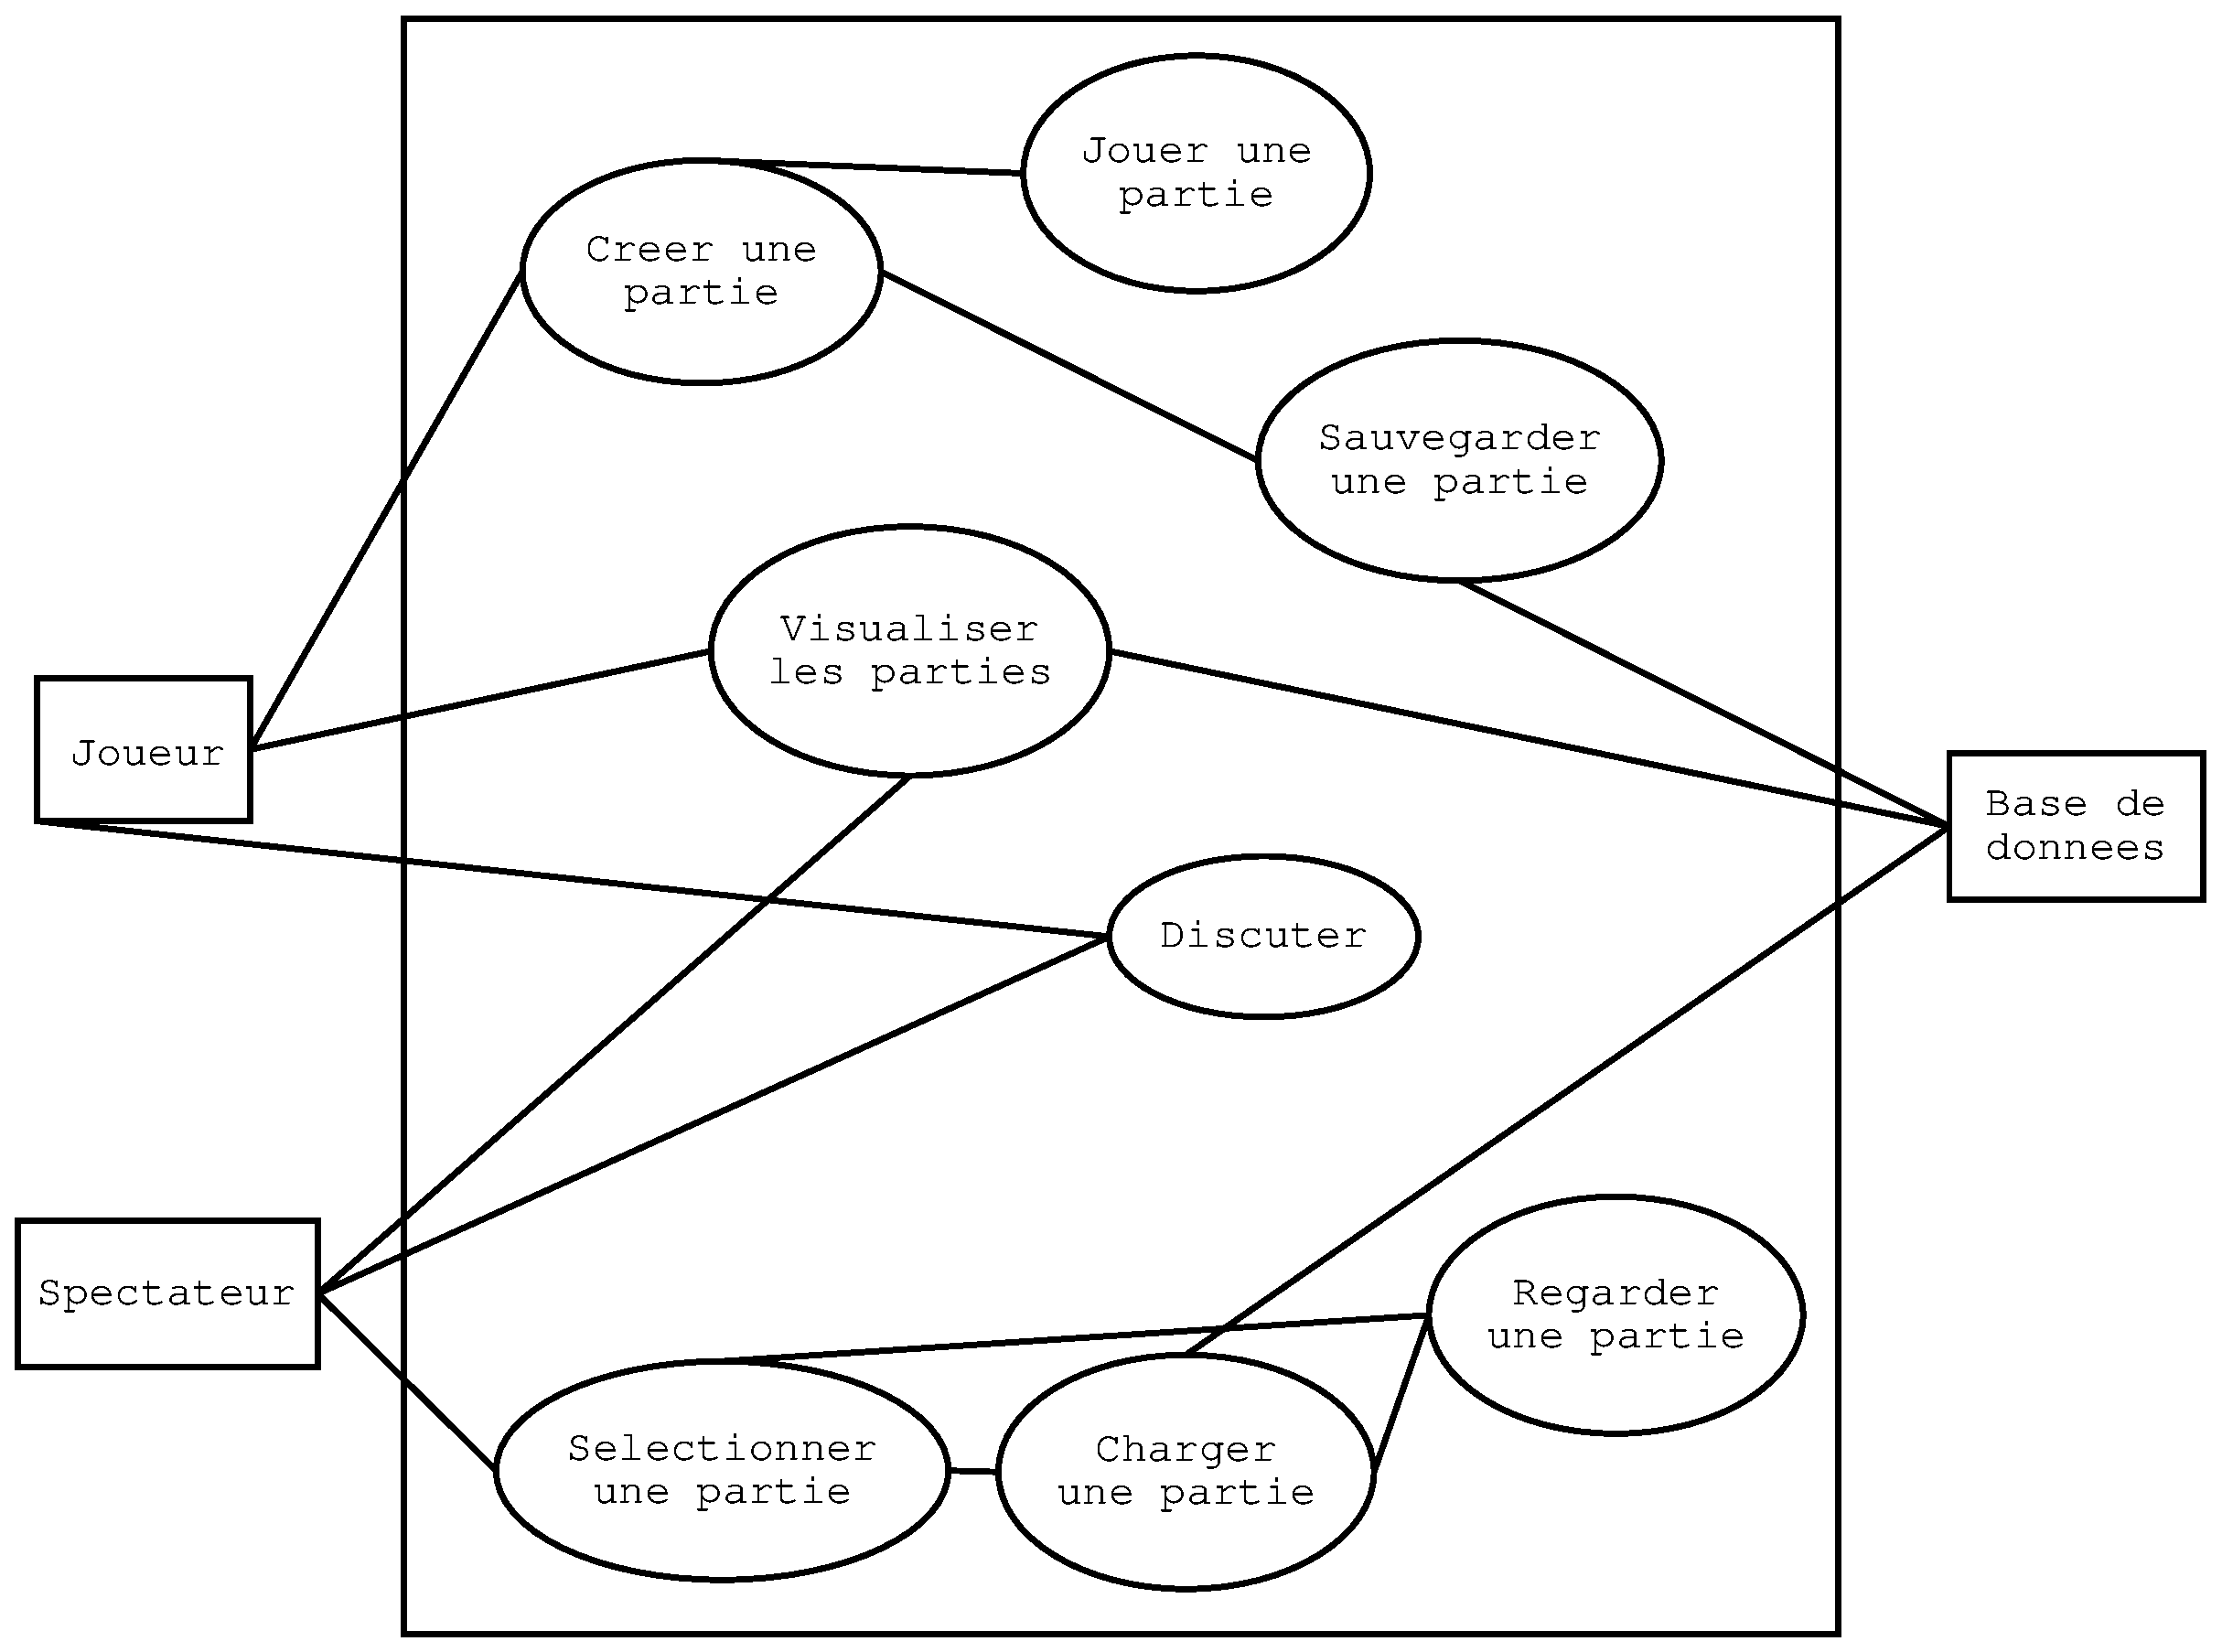
\includegraphics[width=16cm]{DUtilisation2.eps}
\end{figure}

Jeu de dames

\pagebreak

\begin{figure}[!h]
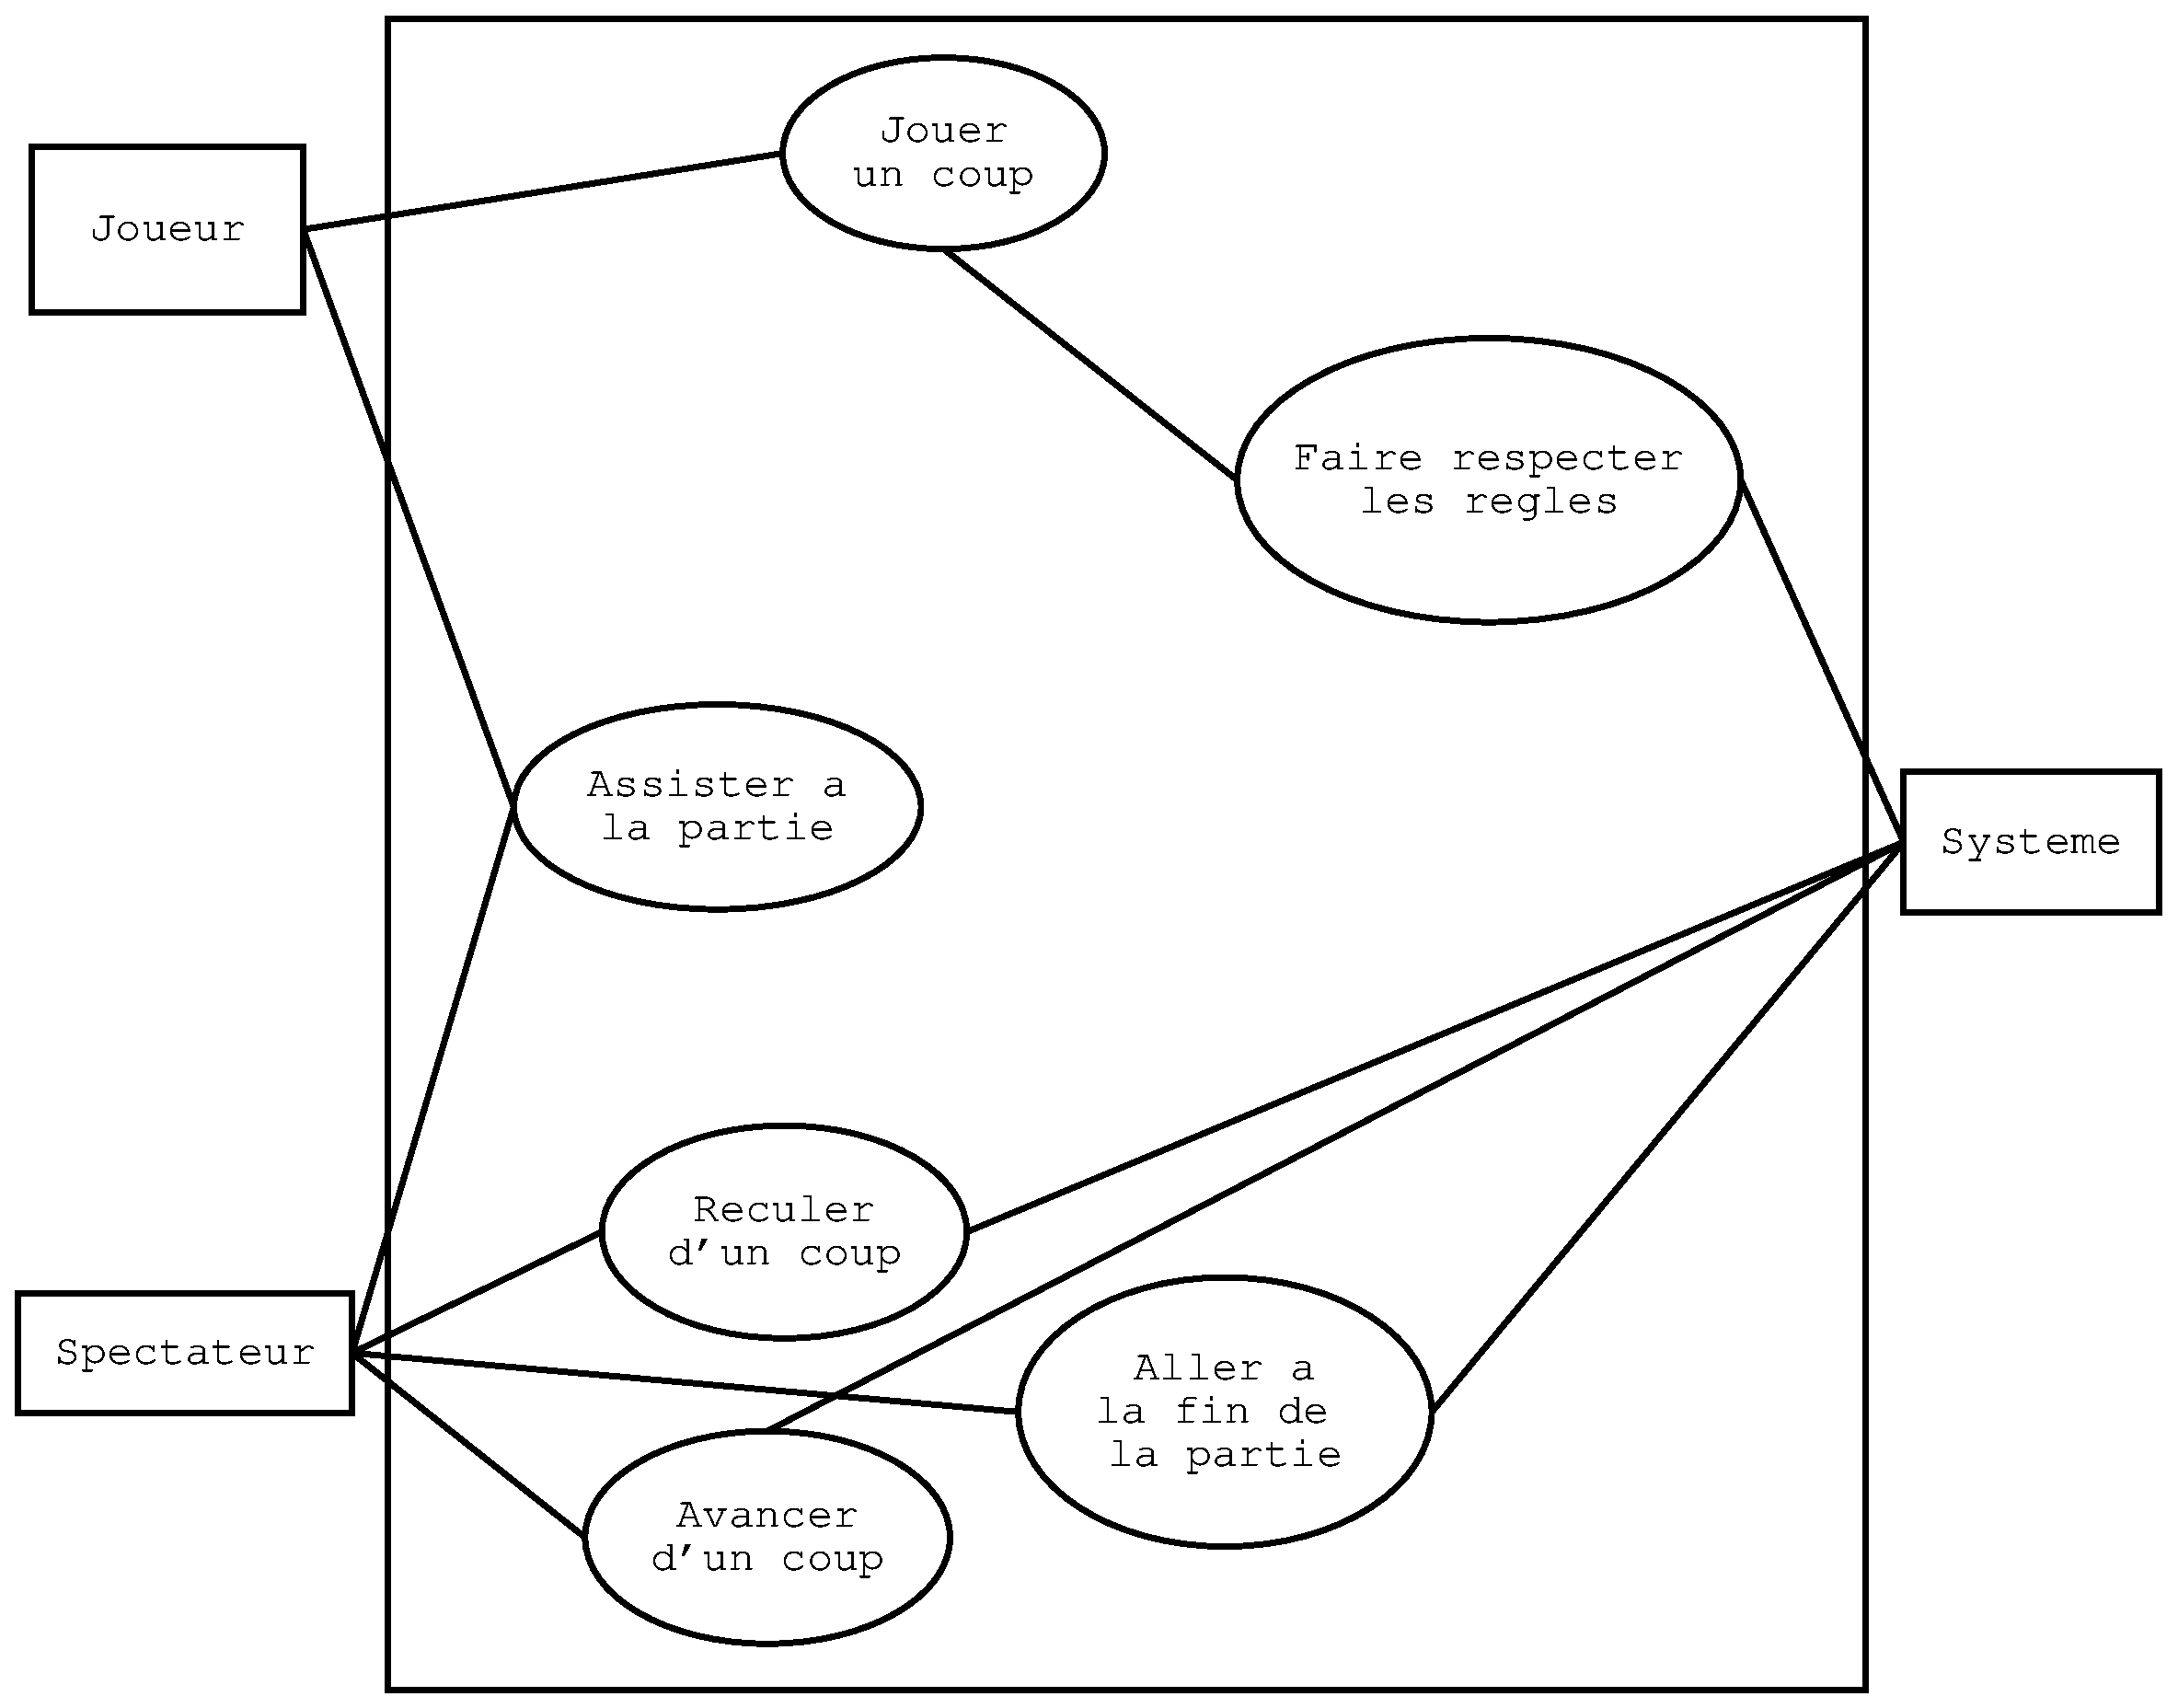
\includegraphics[width=16cm]{DUtilisation1.eps}
\end{figure}

Partie de dames

\end{center}

\pagebreak

\section*{Scenarios}
\addcontentsline{toc}{chapter}{Scenarios}
\markboth{\uppercase{Scenarios}}
{\uppercase{Scenarios}}

\subsection*{Scenario 1}

\begin{tabular}{ll}
  Resum\'e: & un utilisateur veut se connecter au serveur \\
  Acteurs: & utilisateur
\end{tabular}

\paragraph{}
  L'utilisateur lance le client en sp\'ecifiant l'adresse du serveur.
  La connexion est accept\'ee ou refus\'ee, en fonction de l'activit\'e 
du serveur. Si la connexion est accept\'ee, la fen\^etre d'attente 
d'etablissement de connexion se ferme automatiquement et la liste d\'eroulante 
des differentes parties en cours s'affiche dans la fen\^etre principale 
(l'\'ecran d'accueil).



\subsection*{Scenario 2}

\begin{tabular}{ll}
  Resum\'e: & l'utilisateur s'informe des parties actuelles ou pass\'ees \\
  Acteurs: & utilisateur
\end{tabular}

\paragraph{}
  L'utilisateur peut visualiser les parties en cours, ainsi que leurs 
informations (nombres de joueurs, scores ...).
  Il peut egalement charger les parties sauvegard\'ees dans la base de 
donn\'ees. Pour cela, il doit s'engager sur l'onglet 'Charger une partie'. 
Il peut ensuite visualiser les noms des parties pr\'ealablement 
sauvegard\'ees, ainsi que leurs informations.


\subsection*{Scenario 3}

\begin{tabular}{ll}
  Resum\'e: & l'utilisateur veut jouer une partie\\
  Acteurs: & utilisateur(s)
\end{tabular}

\paragraph{}  

  Pour jouer, l'utilisateur peut soit cr\'eer soit rejoindre une partie.

  - Pour cr\'eer une partie, il lui suffit de s'engager sur l'onglet 
'Cr\'eer une partie', de specifier les param\`etres de configuration de sa 
partie, et de cliquer sur le bouton 'Cr\'eer'.
  Le systeme repertorie alors cette partie dans la liste des parties en 
attente de joueur. La partie est en mode attente.

  - Pour rejoindre une partie, l'utilisateur doit double-cliquer sur une 
des parties list\'ees comme \'etant des parties en attente de joueurs 
(sur l'ecran principal).
  Si l'utilisateur est accepte dans la partie, et s'il etait le dernier 
joueur manquant pour demarrer la partie, cette-derniere commence.



\subsection*{Scenario 4}

\begin{tabular}{ll}
  Resum\'e: & l'utilisateur souhaite visualiser une partie en deroulement \\
  Acteurs: & utilisateur \\
	   & BD
\end{tabular}

\paragraph{}
  L'utilisateur veut visualiser une partie en cours ou pass\'ees. 
  Il clique sur l'onglet 'Visualiser une partie'. La liste des parties 
  visualisable s'affiche alors. L'utilisateur choisit une partie \'a partir 
  de leur description (en cours de jeu, noms des joueurs...). 
  Il double-clique sur celle de son choix et y accede.



\subsection*{Scenario 5}

\begin{tabular}{ll}
  Resum\'e: & le joueur joue un coup \\
  Acteurs: & joueur
\end{tabular}

\paragraph{}    
  Le joueur joue un coup. Pour cela, il s\'electionne d'un clique la case 
qui contient le pion qu'il d\'esire deplacer. Il clique ensuite sur la 
case de destination.
  Le client interroge alors le serveur pour verifier la validit\'e du coup.
  Si le coup est valide, il est accepte et joue, sinon, le joueur a de 
nouveau la main pour proposer un autre coup.
  Si, d'autre part, le coup etait gagnant, la partie se termine.



\subsection*{Scenario 6}

\begin{tabular}{ll}
  Resum\'e: & l'utilisateur quitte la partie \\
  Acteurs: & utilisateur
\end{tabular}

\paragraph{}    
  Le joueur veut quitter la partie. Il clique sur le bouton 'Abandonner'.
  Une boite de dialogue s'affiche lui proposant de sauvegarder la partie. 
L'utilisateur accepte ou refuse.
  Une nouvelle boite de dialogue lui demande une confirmation pour quitter 
le jeu. Si l'utilisateur confirme, il est declare perdant et revient \'a la 
fenetre d'acceuil; sinon la partie reprend.




\subsection*{Scenario 7}

\begin{tabular}{ll}
  Resum\'e: & l'adversaire quitte la partie \\
  Acteurs: & adversaire
	     joueur
\end{tabular}

\paragraph{}   
  Si l'adversaire quitte la partie, le joueur est declare vainqueur et 
il revient automatiquement \'a la fenetre d'accueil.



\subsection*{Scenario 8}

\begin{tabular}{ll}
  Resum\'e: & sauvegarder une partie \\
  Acteurs: & joueur \\
	   & BD
\end{tabular}

\paragraph{}    
  En pleine partie, le joueur peut sauvegarder l'etat du jeu. Pour cela, 
il clique sur le bouton 'Sauvegarder'. La liste des parties qu'il a deja 
enregistr\'ees s'affiche alors. Il choisit d'\'ecraser une ancienne 
sauvegarde ou de cr\'eer un nouvelle enregistrement. 
  S'il cr\'ee un nouvelle enregistrement, une boite de dialogue lui demande 
alors un nom pour cette sauvegarde.
  S'il \'ecrase un ancien enregistrement, une boite de dialogue lui demande 
de confirmer cette action.
  L'\'etat de la partie est alors enregistr\'e dans la base de donnees.


\subsection*{Scenario 9}

\begin{tabular}{ll}
  Resum\'e: & l'utilisateur veut charger une partie \\
  Acteurs: & joueur \\
	   & BD
\end{tabular}

\paragraph{} 
  Depuis la liste des parties sauvegard\'ees, dans l'onglet 
'Charger une partie', l'utilisateur s\'electionne une partie de la base 
de donn\'ees d'un double-clique et la charge.
  La partie est alors repertori\'ee comme une partie en attente de joueur..



\subsection*{Scenario 10}

\begin{tabular}{ll}
  Resum\'e : l'utilisateur veut avancer la partie au coup suivant
  Acteurs : utilisateur
\end{tabular}

\paragraph{}
  L'utilisateur clique sur le bouton (en forme de fl\`eche vers la droite) 
permettant d'avancer la partie au coup suivant.
  Le client envoie la demande au serveur qui retourne au client le coup a 
jou\'e. Le client affiche les changements sur l'aire de jeu.



\subsection*{Scenario 11}

\begin{tabular}{ll}
  Resum\'e: & l'utilisateur veut revenir d'un coup en arriere dans la partie \\
  Acteurs: & utilisateur
\end{tabular}

\paragraph{}
  L'utilisateur clique sur le bouton (en forme de fl\`eche vers la gauche) 
permettant de revenir un coup en arri\`ere dans la partie.
  Le client envoie la demande au serveur qui retourne au client la 
position precedente.
  Le client affiche les changements sur l'aire de jeu.



\subsection*{Scenario 12}

\begin{tabular}{ll}
  Resum\'e: & l'utilisateur veut avancer dans la partie jusqu'au dernier 
coup \\
  Acteurs: & utilisateur
\end{tabular}

\paragraph{}
  L'utilisateur clique sur le bouton (en forme de double-fl\`eche vers la 
droite) permettant d'avancer dans la partie jusau'au dernier coup de la partie.
  Le client envoie la demande au serveur qui retourne au client la 
liste de tout les coups suivants.
  Le client affiche le premier coup et attend l'autorisation de 
l'utilisateur pour afficher le coup d'apr\`es.
  L'utilisateur \`a \'egalement la possibilite d'affichager directement 
le dernier coup.



\subsection*{Scenario 13}

\begin{tabular}{ll}
  Resum\'e: & l'utilisateur veut revenir au debut de la partie \\
  Acteurs: & utilisateur
\end{tabular}

\paragraph{} 
  L'utilisateur clique sur le bouton (en forme de double-fleche 
vers la gauche) permettant de revenir au premier coup de la partie.
  Le client envoie la demande au serveur qui retourne au client 
les positions initiales des pions.
  Le client affiche les changements sur l'aire de jeu.

\pagebreak

\section*{Diagramme de composant}
\addcontentsline{toc}{chapter}{Diagramme de composant}
\markboth{\uppercase{Diagrammes de composants}}
{\uppercase{Diagrammes de composants}}

\begin{center}
\begin{figure}[h]
\includegraphics[width=16cm]{DdeC.eps}
\end{figure}

Diagramme de composant
\end{center}

On note ici que le client n'a aucune notion de r\`egles. Elles sont toutes
stock\'ees sur le serveur. Seule la maniere d'afficher le plateau
ainsi que les pions est conserv\'ee.

\pagebreak

\section*{Diagrammes d'activit\'es}
\addcontentsline{toc}{chapter}{Diagrammes d'activit\'es}
\markboth{\uppercase{Diagrammes d'activit\'es}}
{\uppercase{Diagrammes d'activit\'es}}

\begin{center}
\begin{figure}[h]
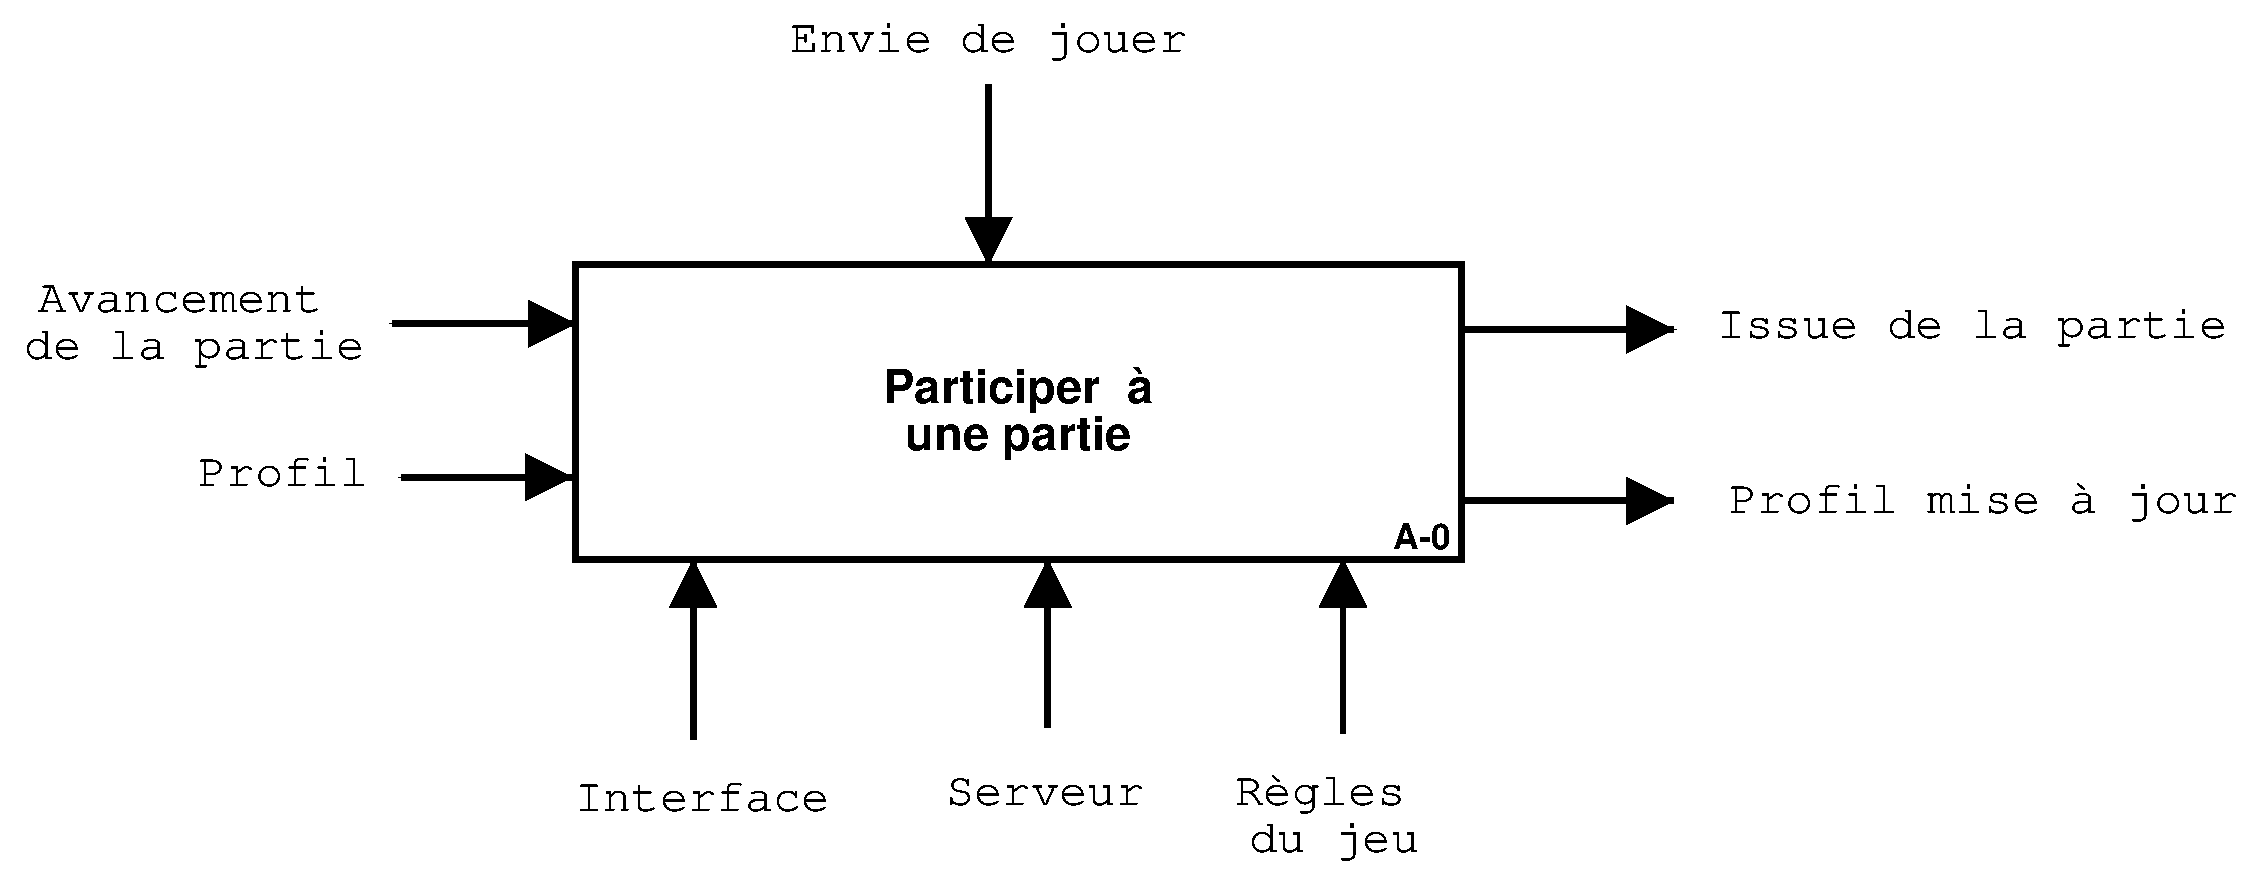
\includegraphics[width=16cm]{A-0.eps}
\end{figure}

Participer a une partie

\pagebreak

\begin{figure}[h]
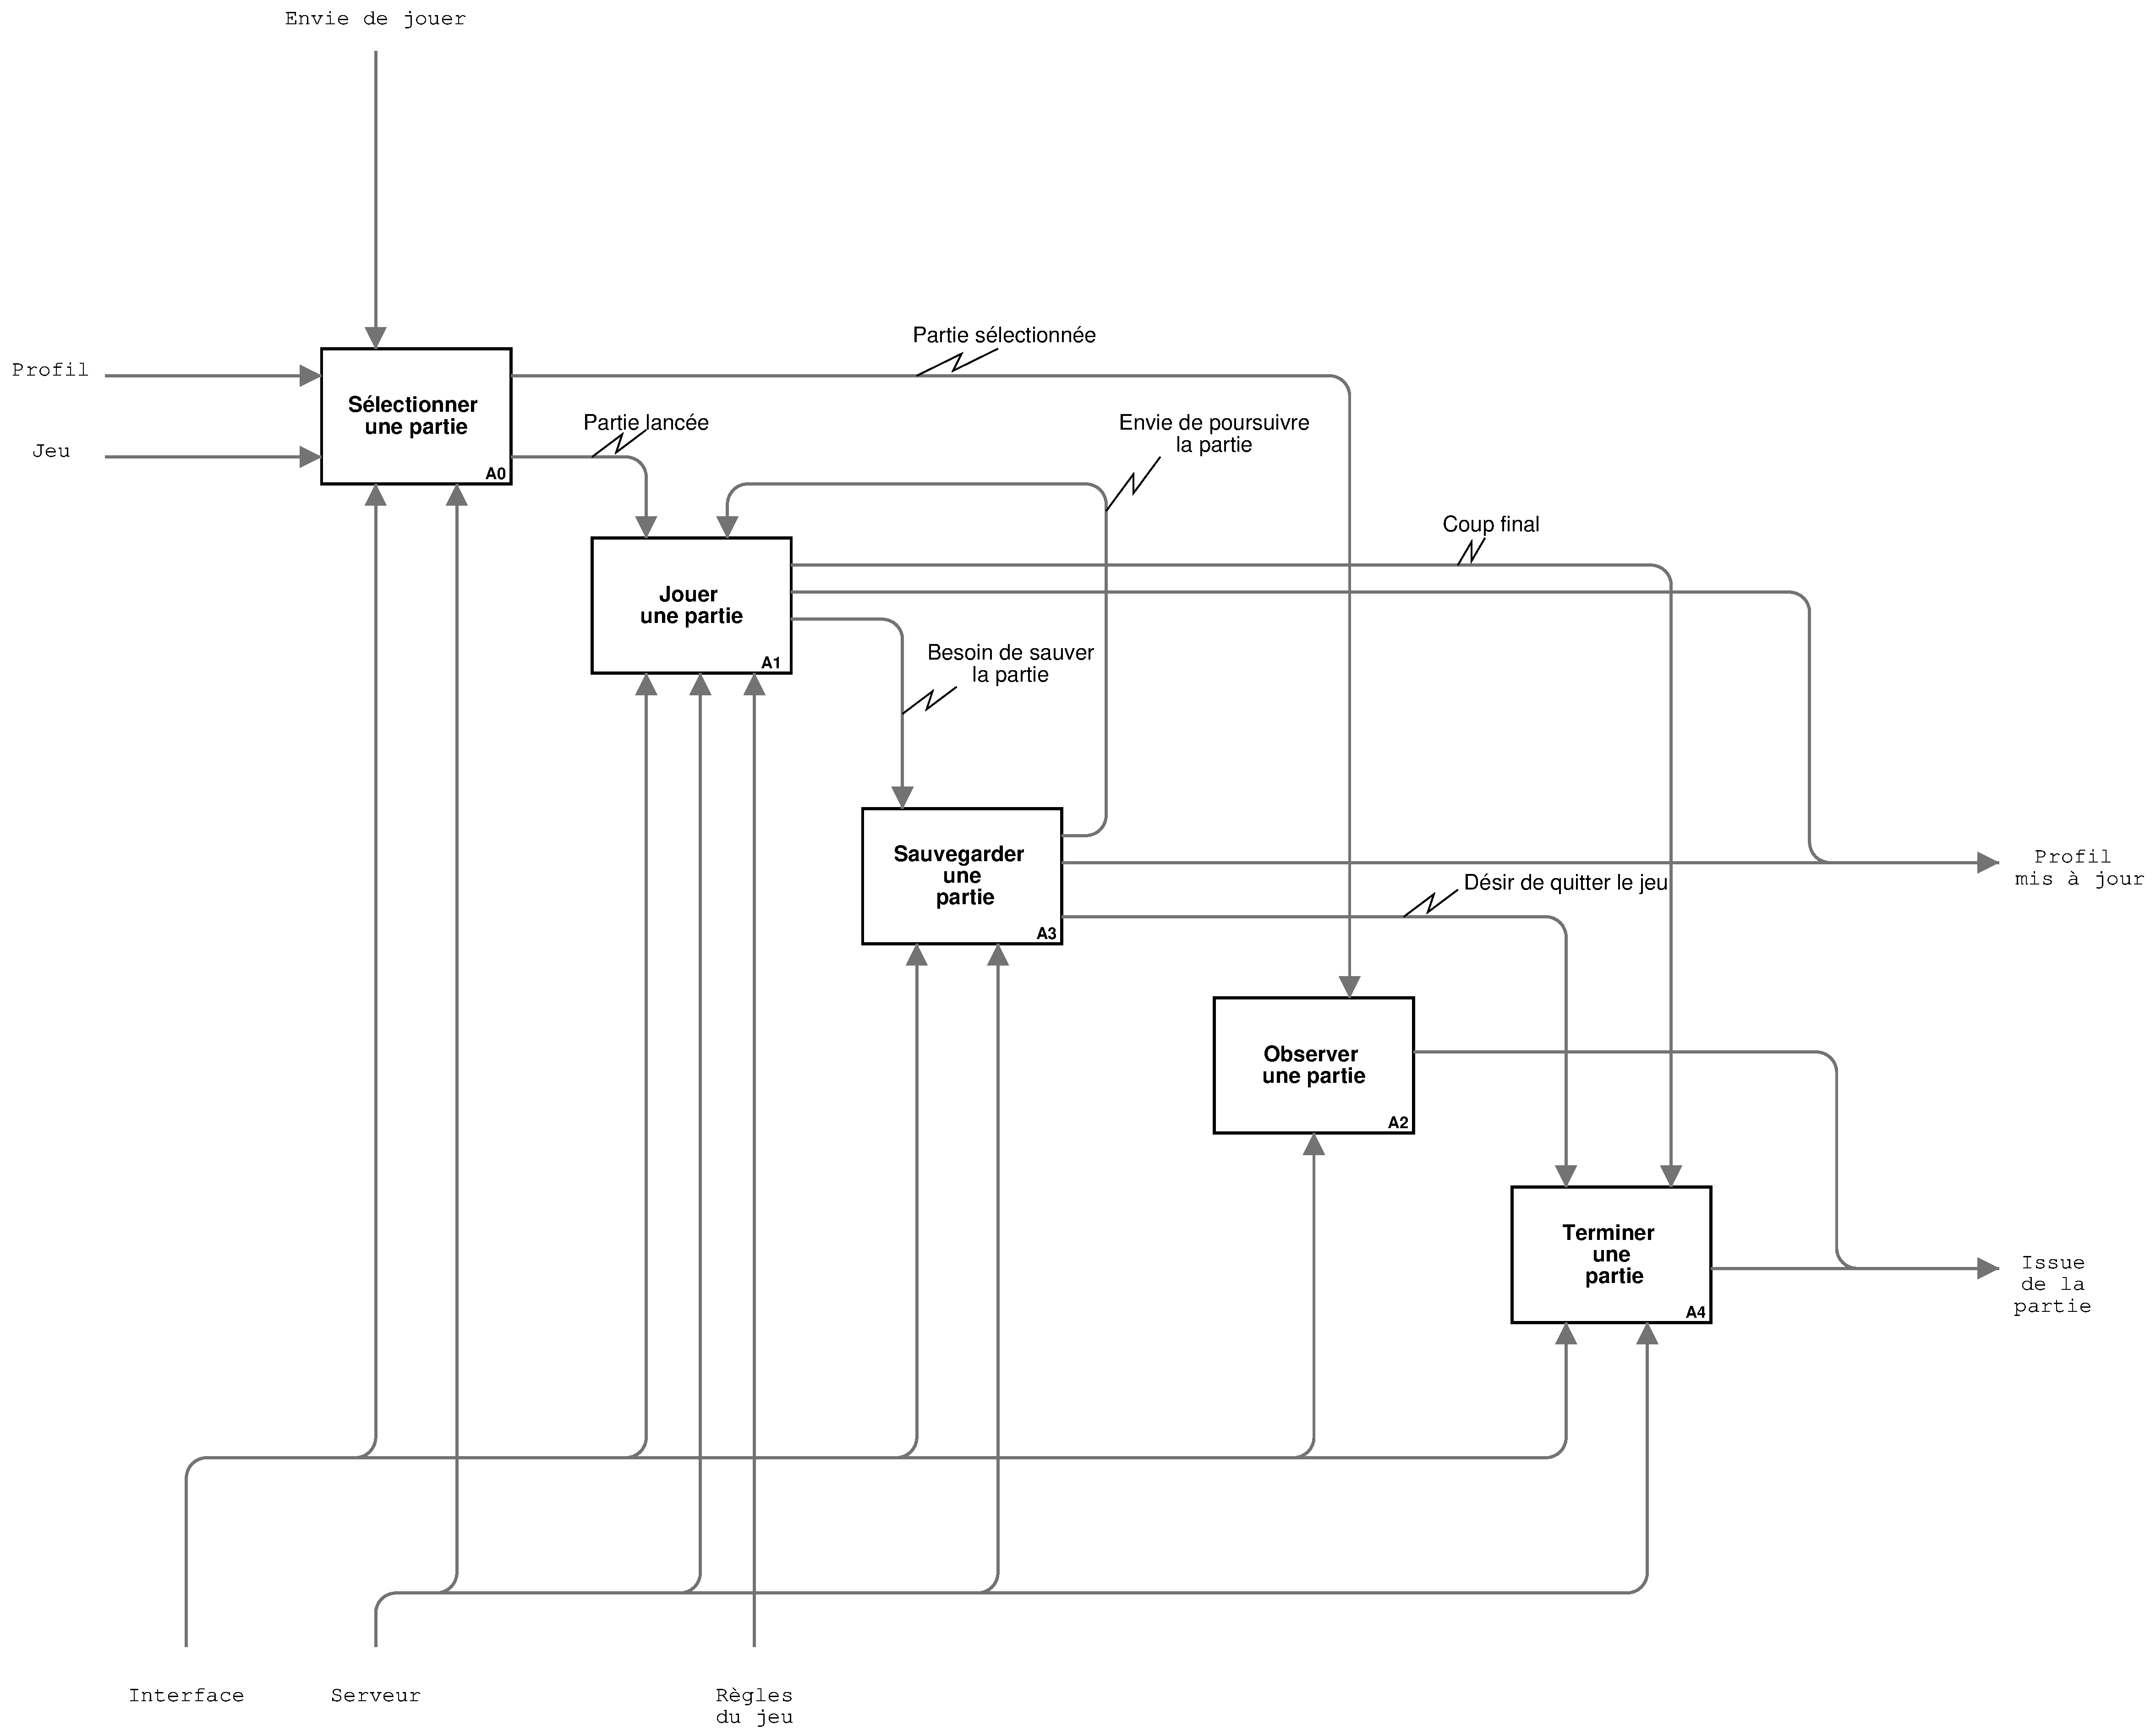
\includegraphics[width=16cm]{A0.eps}
\end{figure}

Participer a une partie

\pagebreak

\begin{figure}[h]
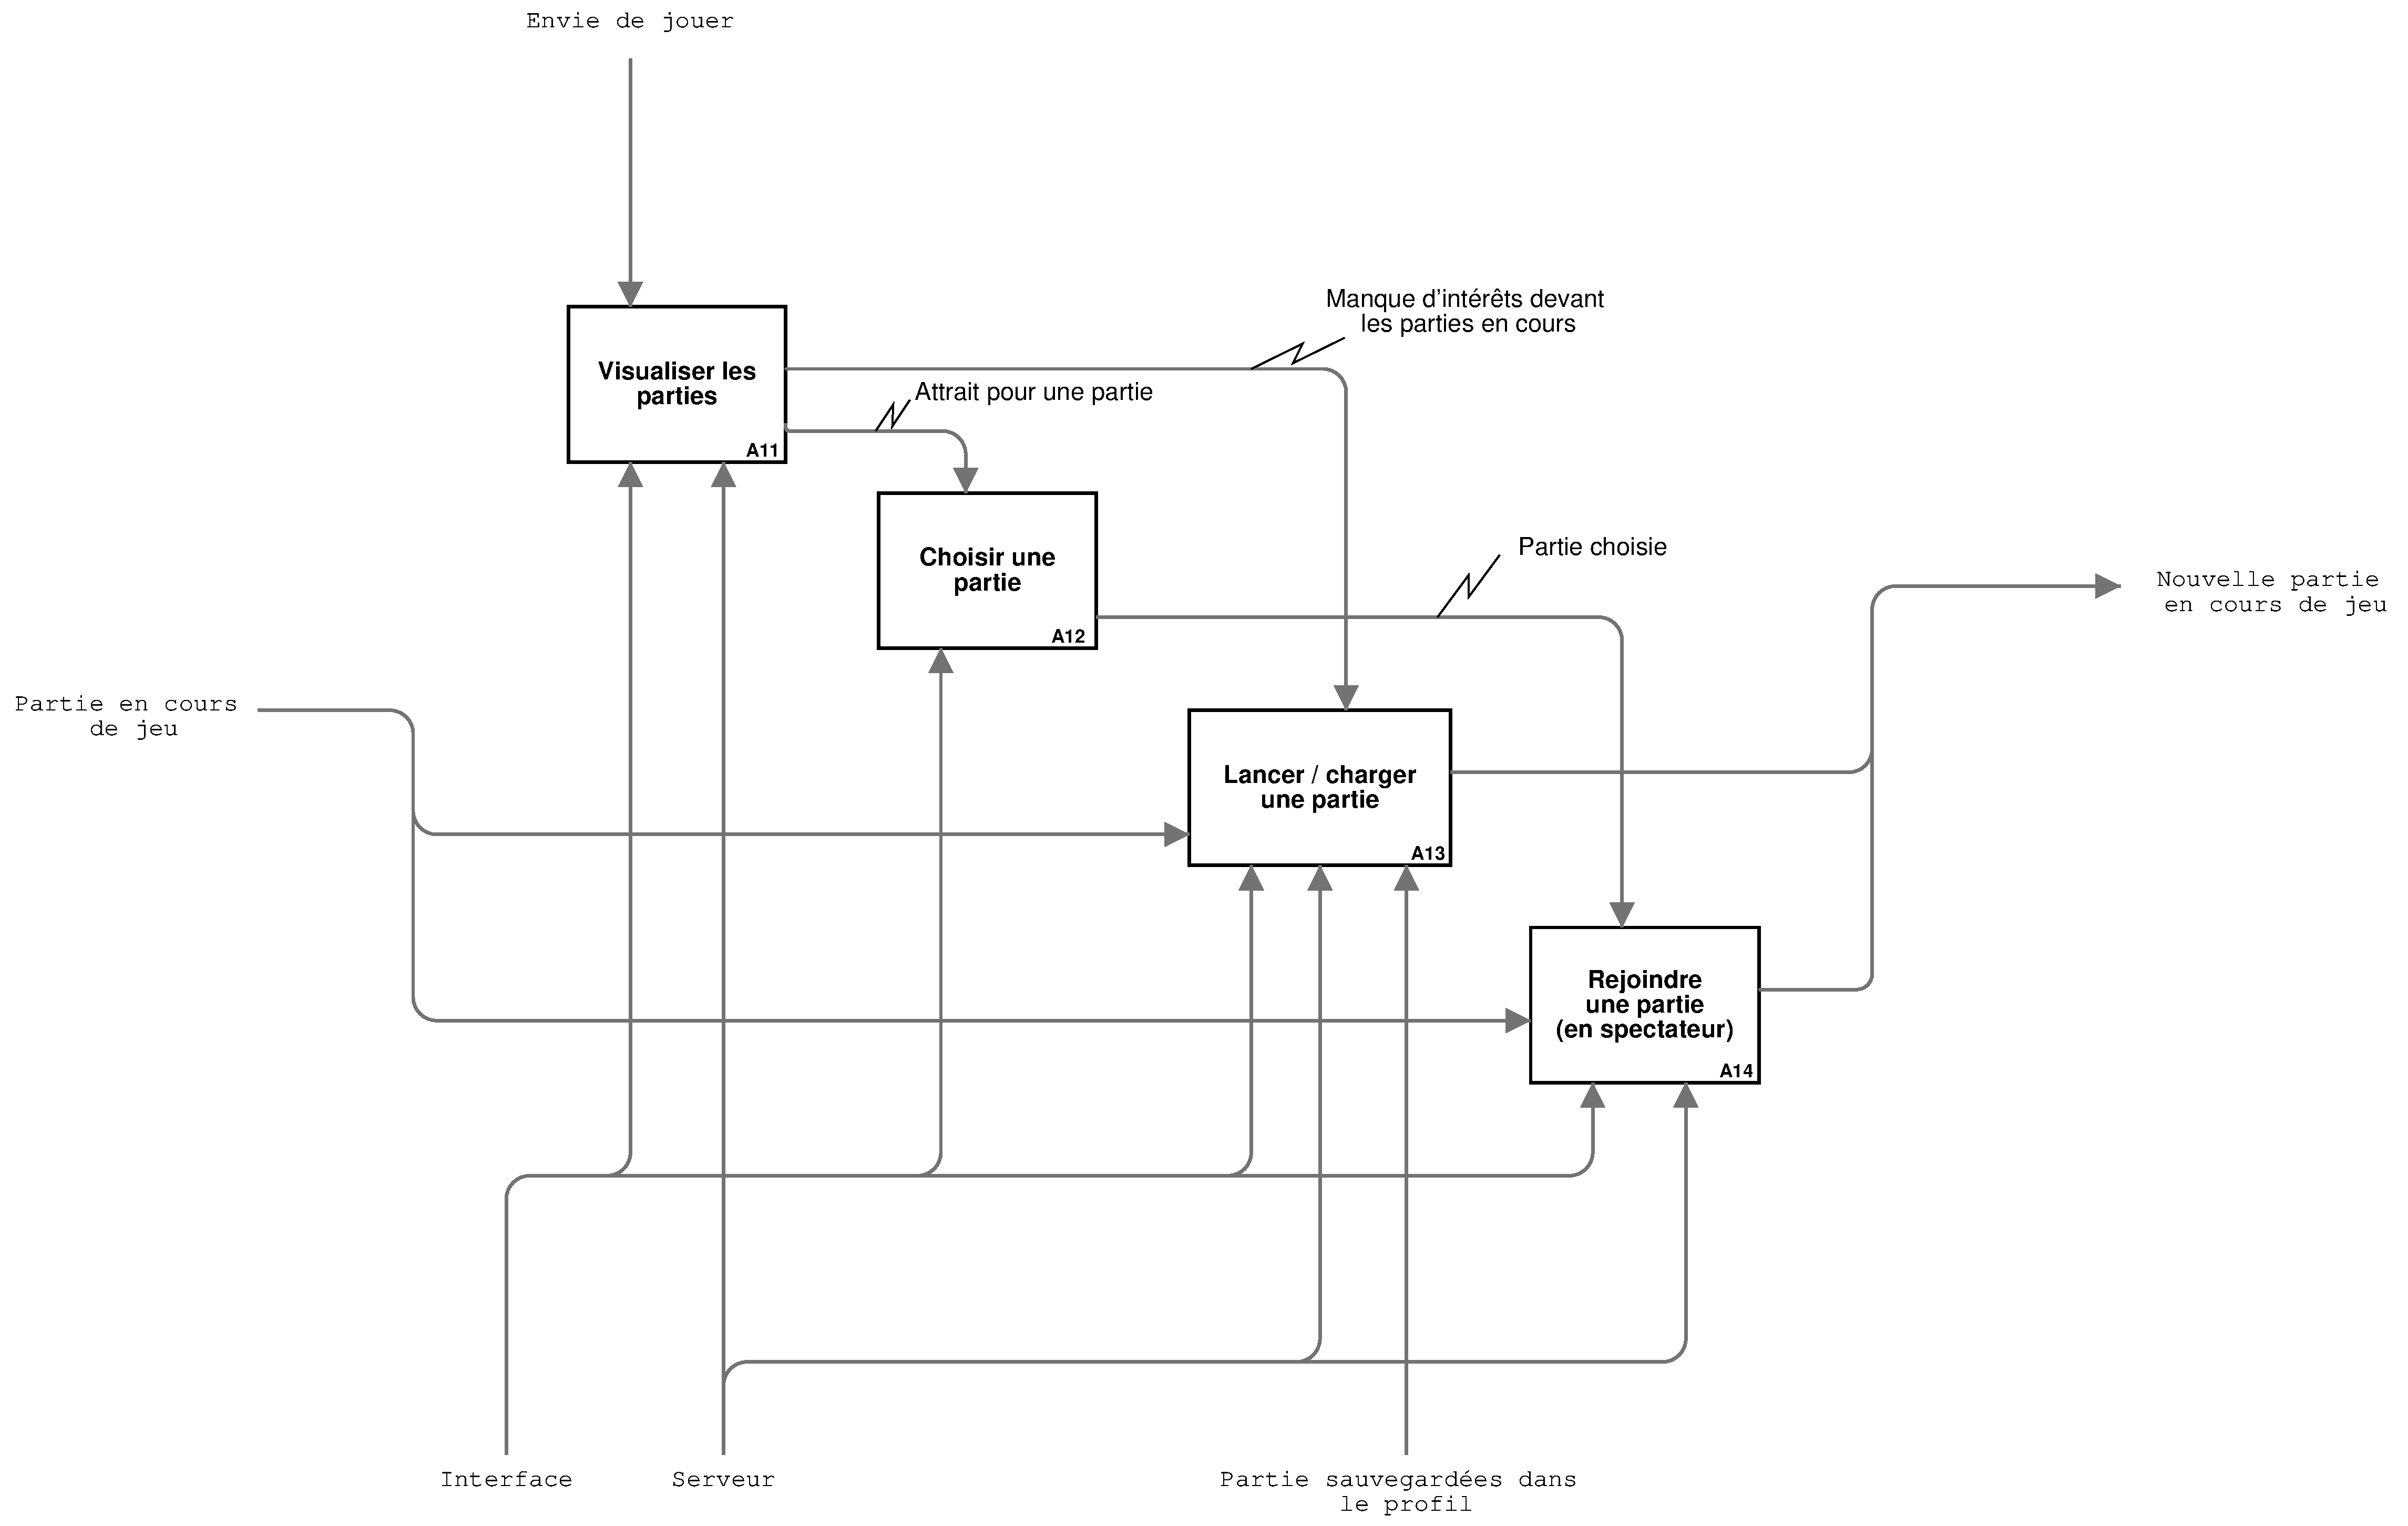
\includegraphics[width=16cm]{A1.eps}
\end{figure}

Selectionner une partie

\pagebreak

\begin{figure}[h]
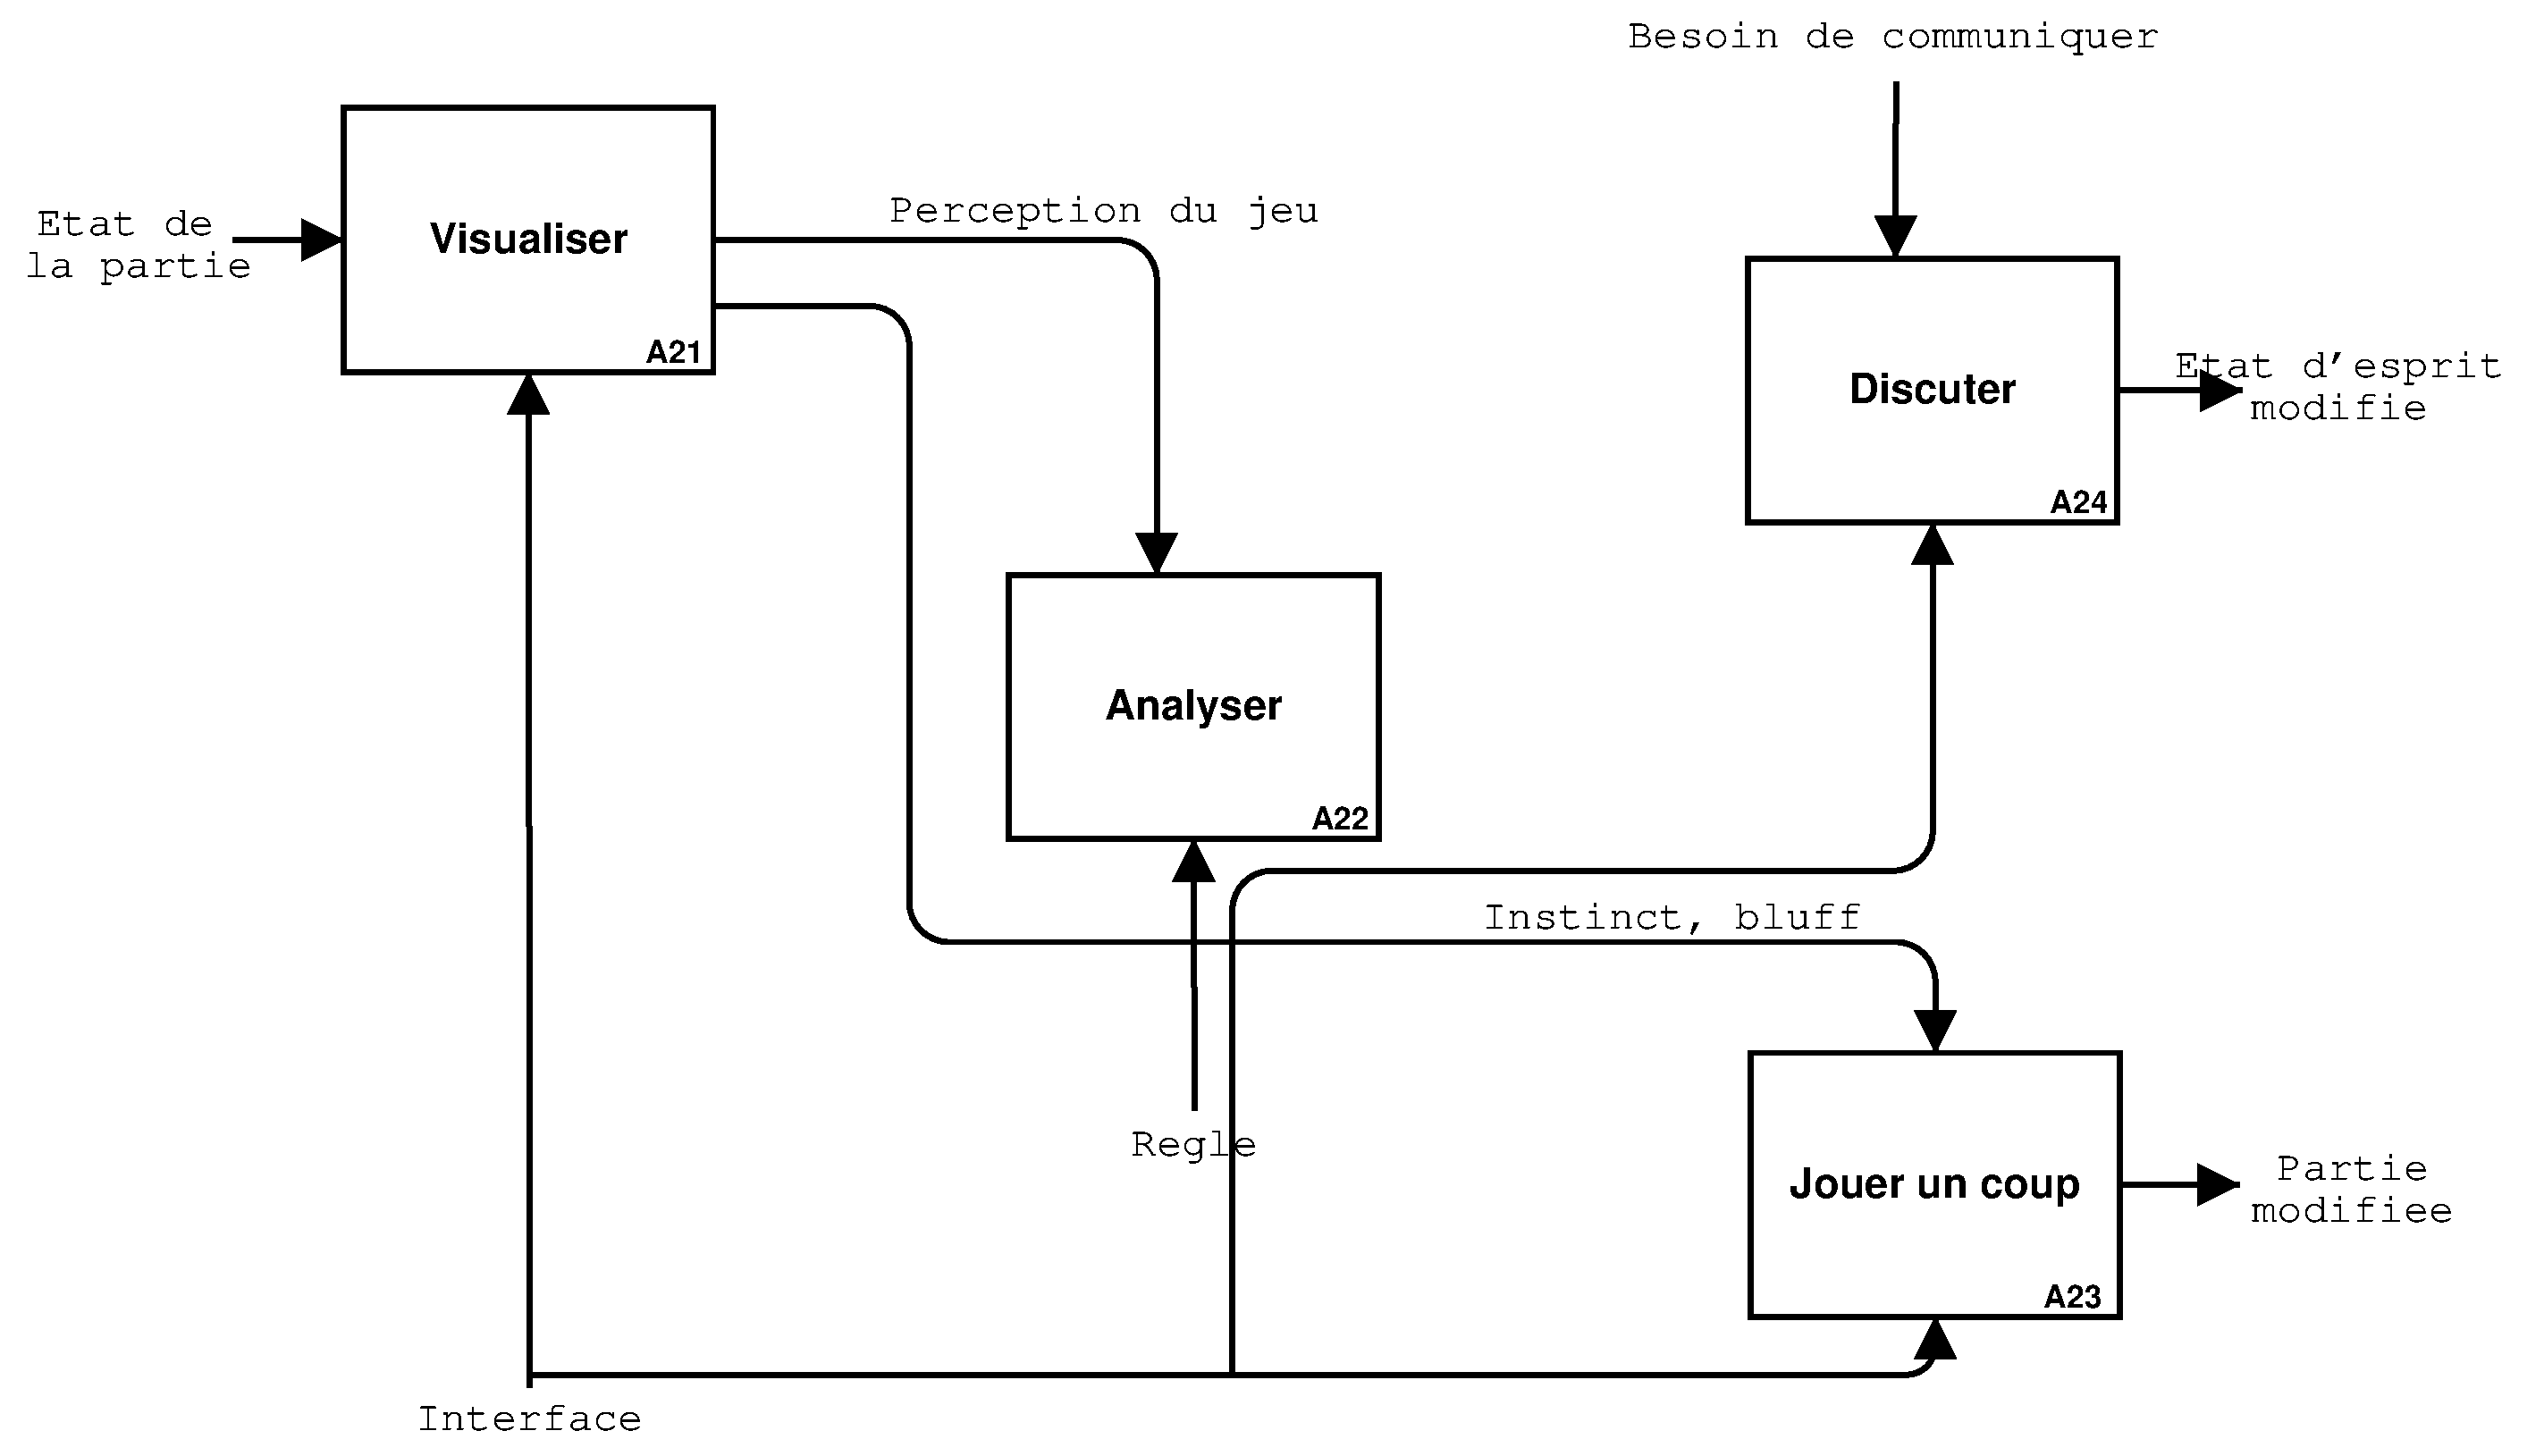
\includegraphics[width=16cm]{A2.eps}
\end{figure}

Jouer

\pagebreak

\begin{figure}[h]
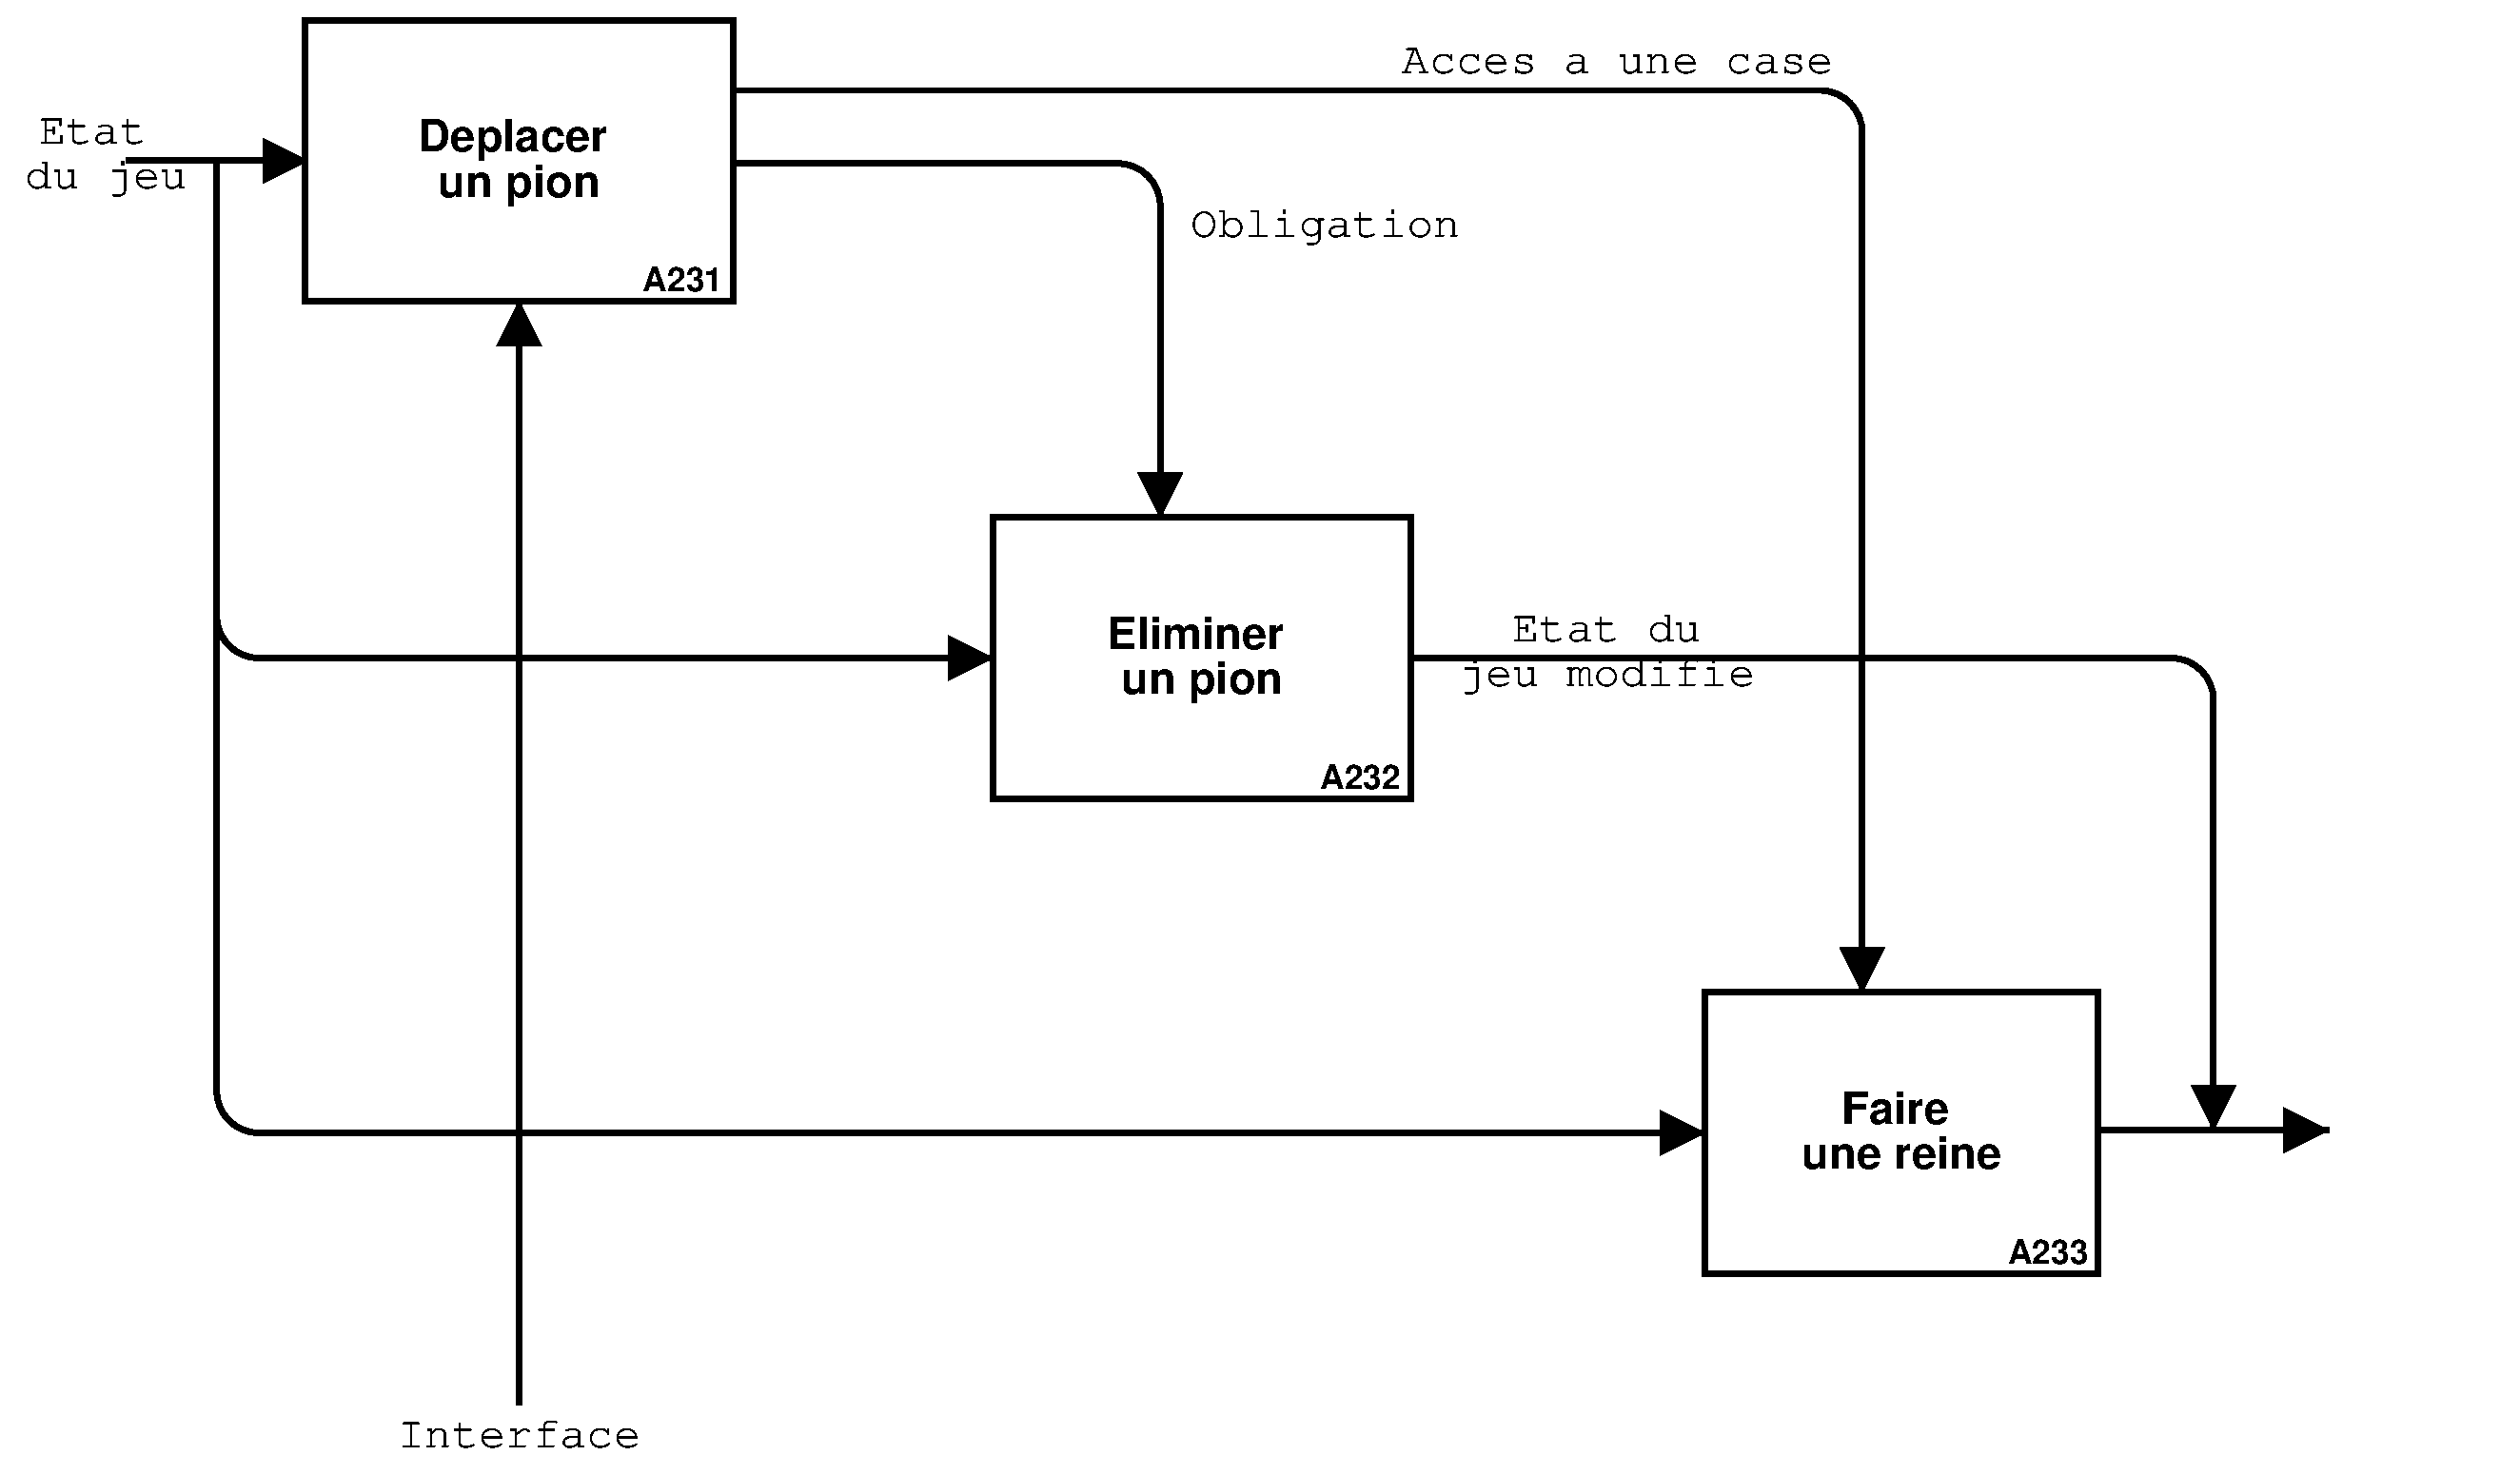
\includegraphics[width=16cm]{A23.eps}
\end{figure}

Jouer un coup

\pagebreak

\begin{figure}[h]
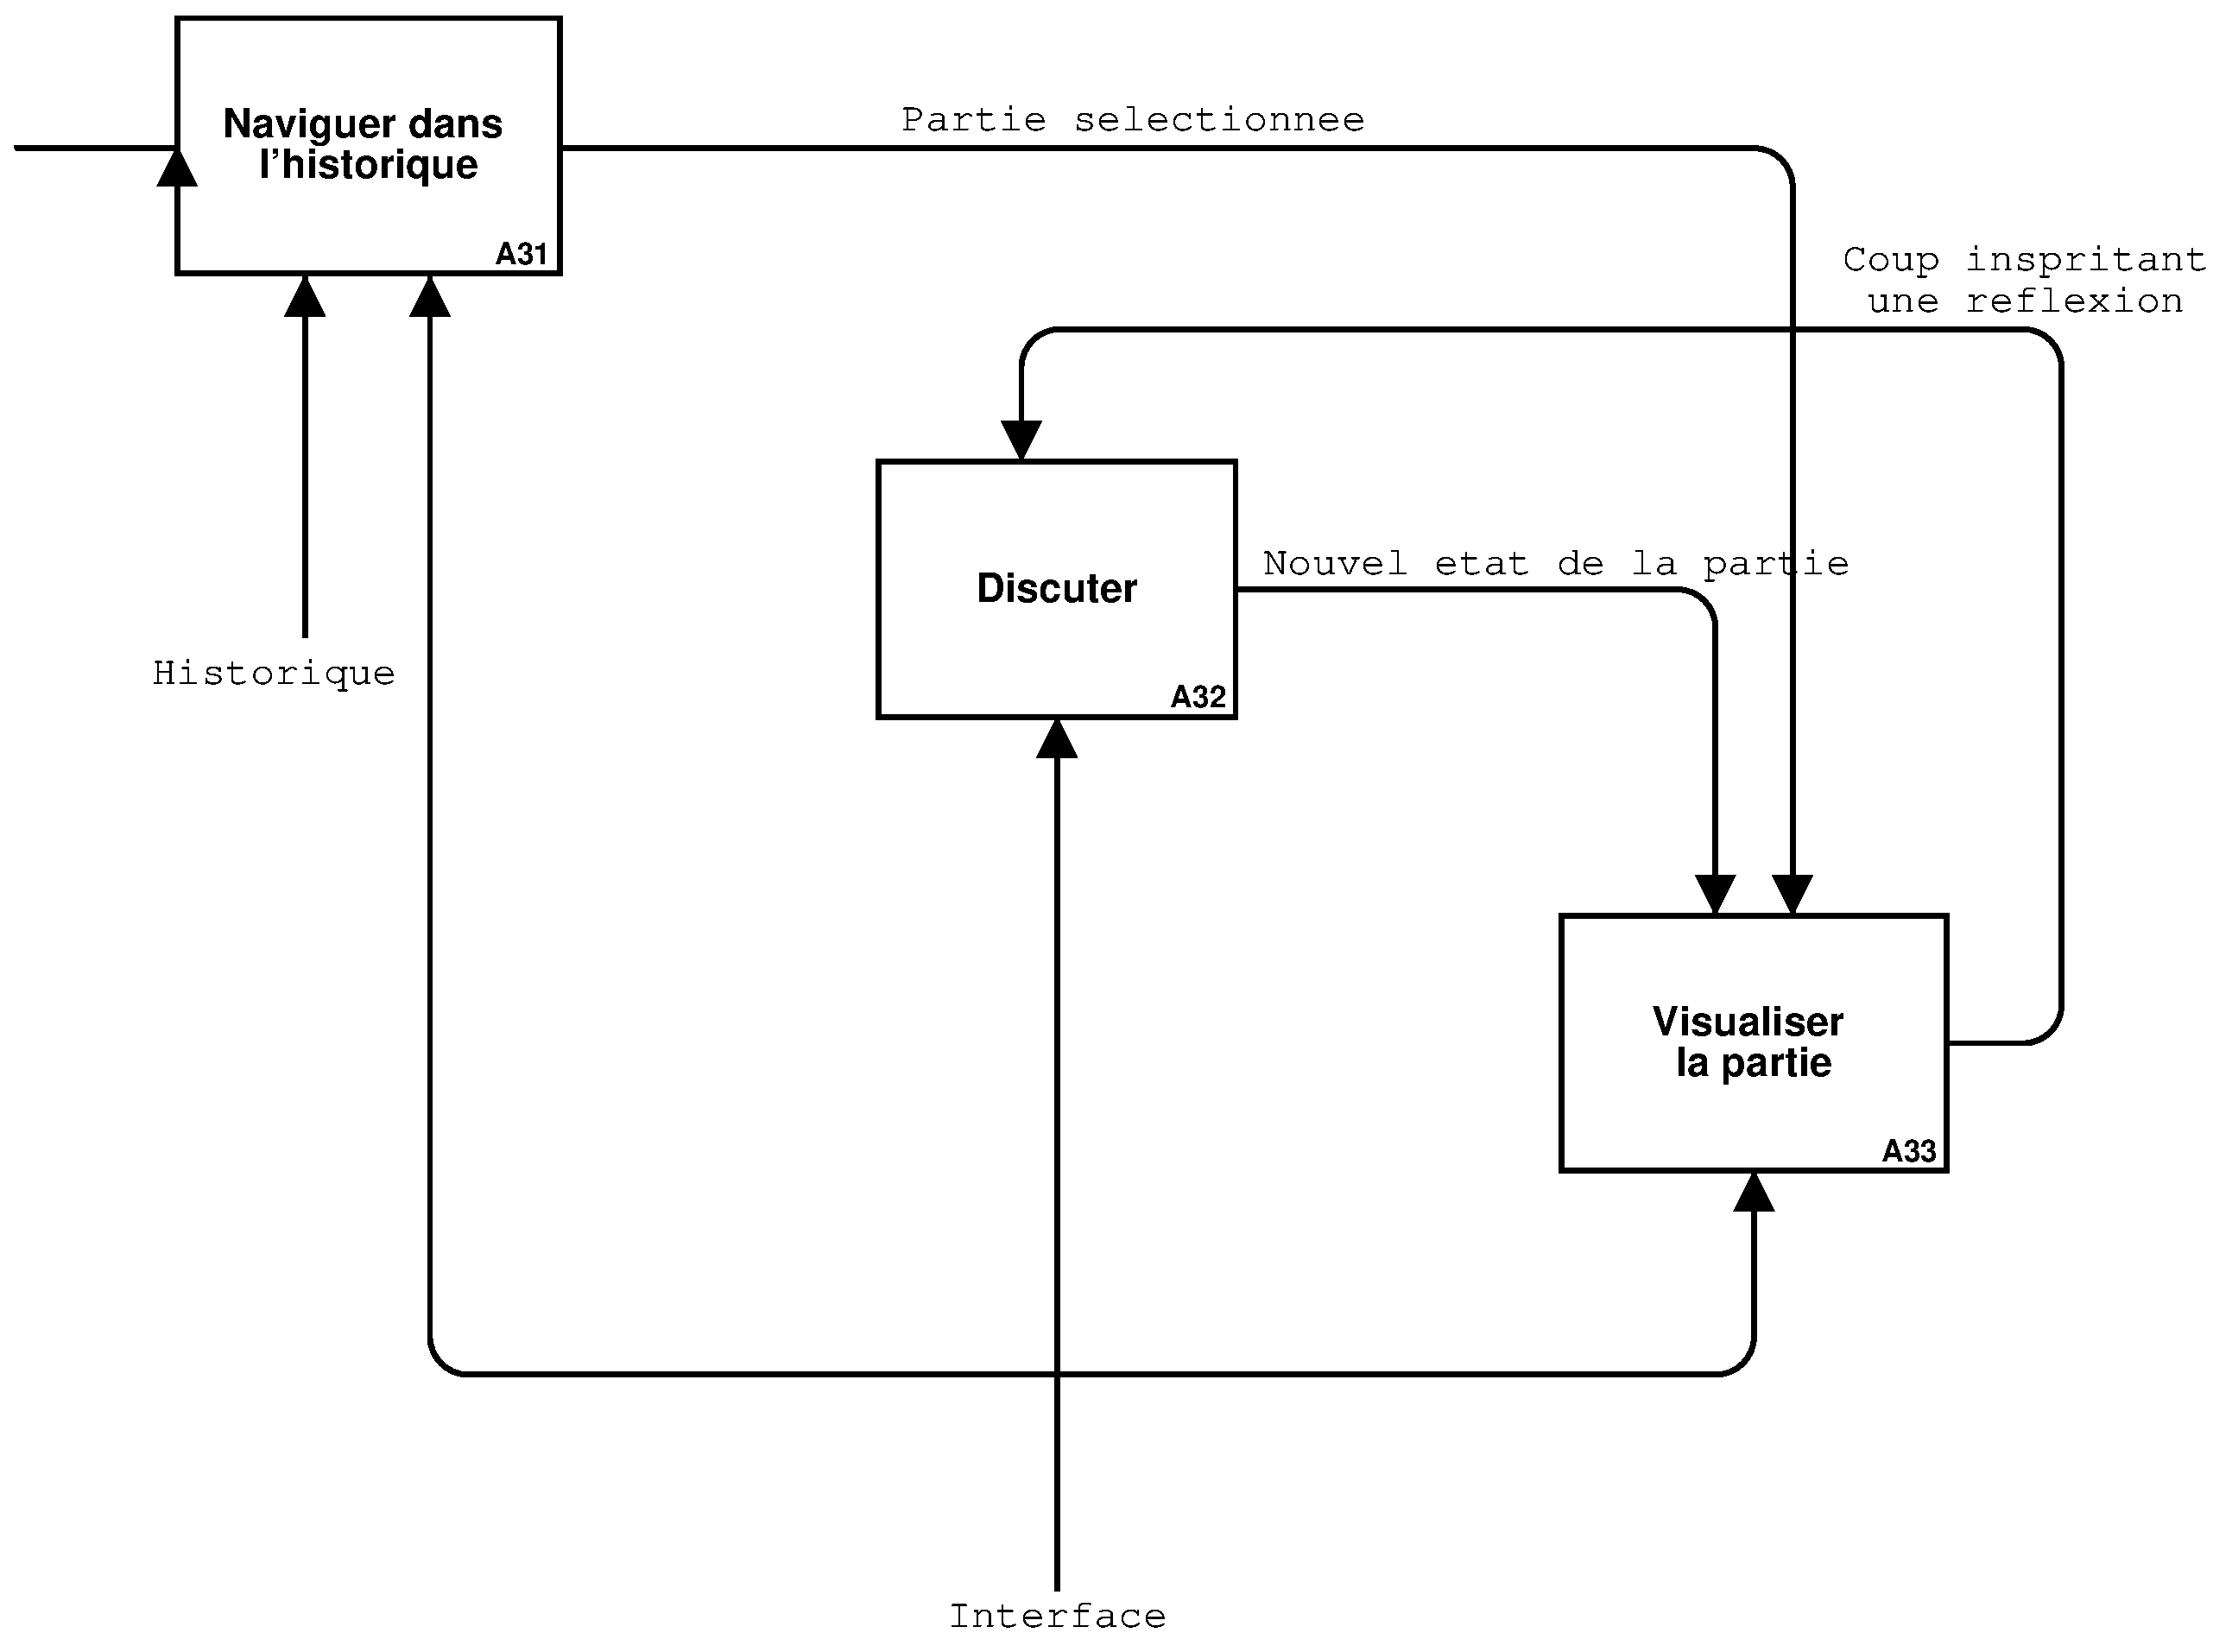
\includegraphics[width=16cm]{A3.eps}
\end{figure}

Observer

\end{center}

\pagebreak

\section*{Diagrammes de classes}
\addcontentsline{toc}{chapter}{Diagrammes de classes}
\markboth{\uppercase{Diagrammes de classes}}
{\uppercase{Diagrammes de classes}}

\begin{center}

\begin{figure}[h]
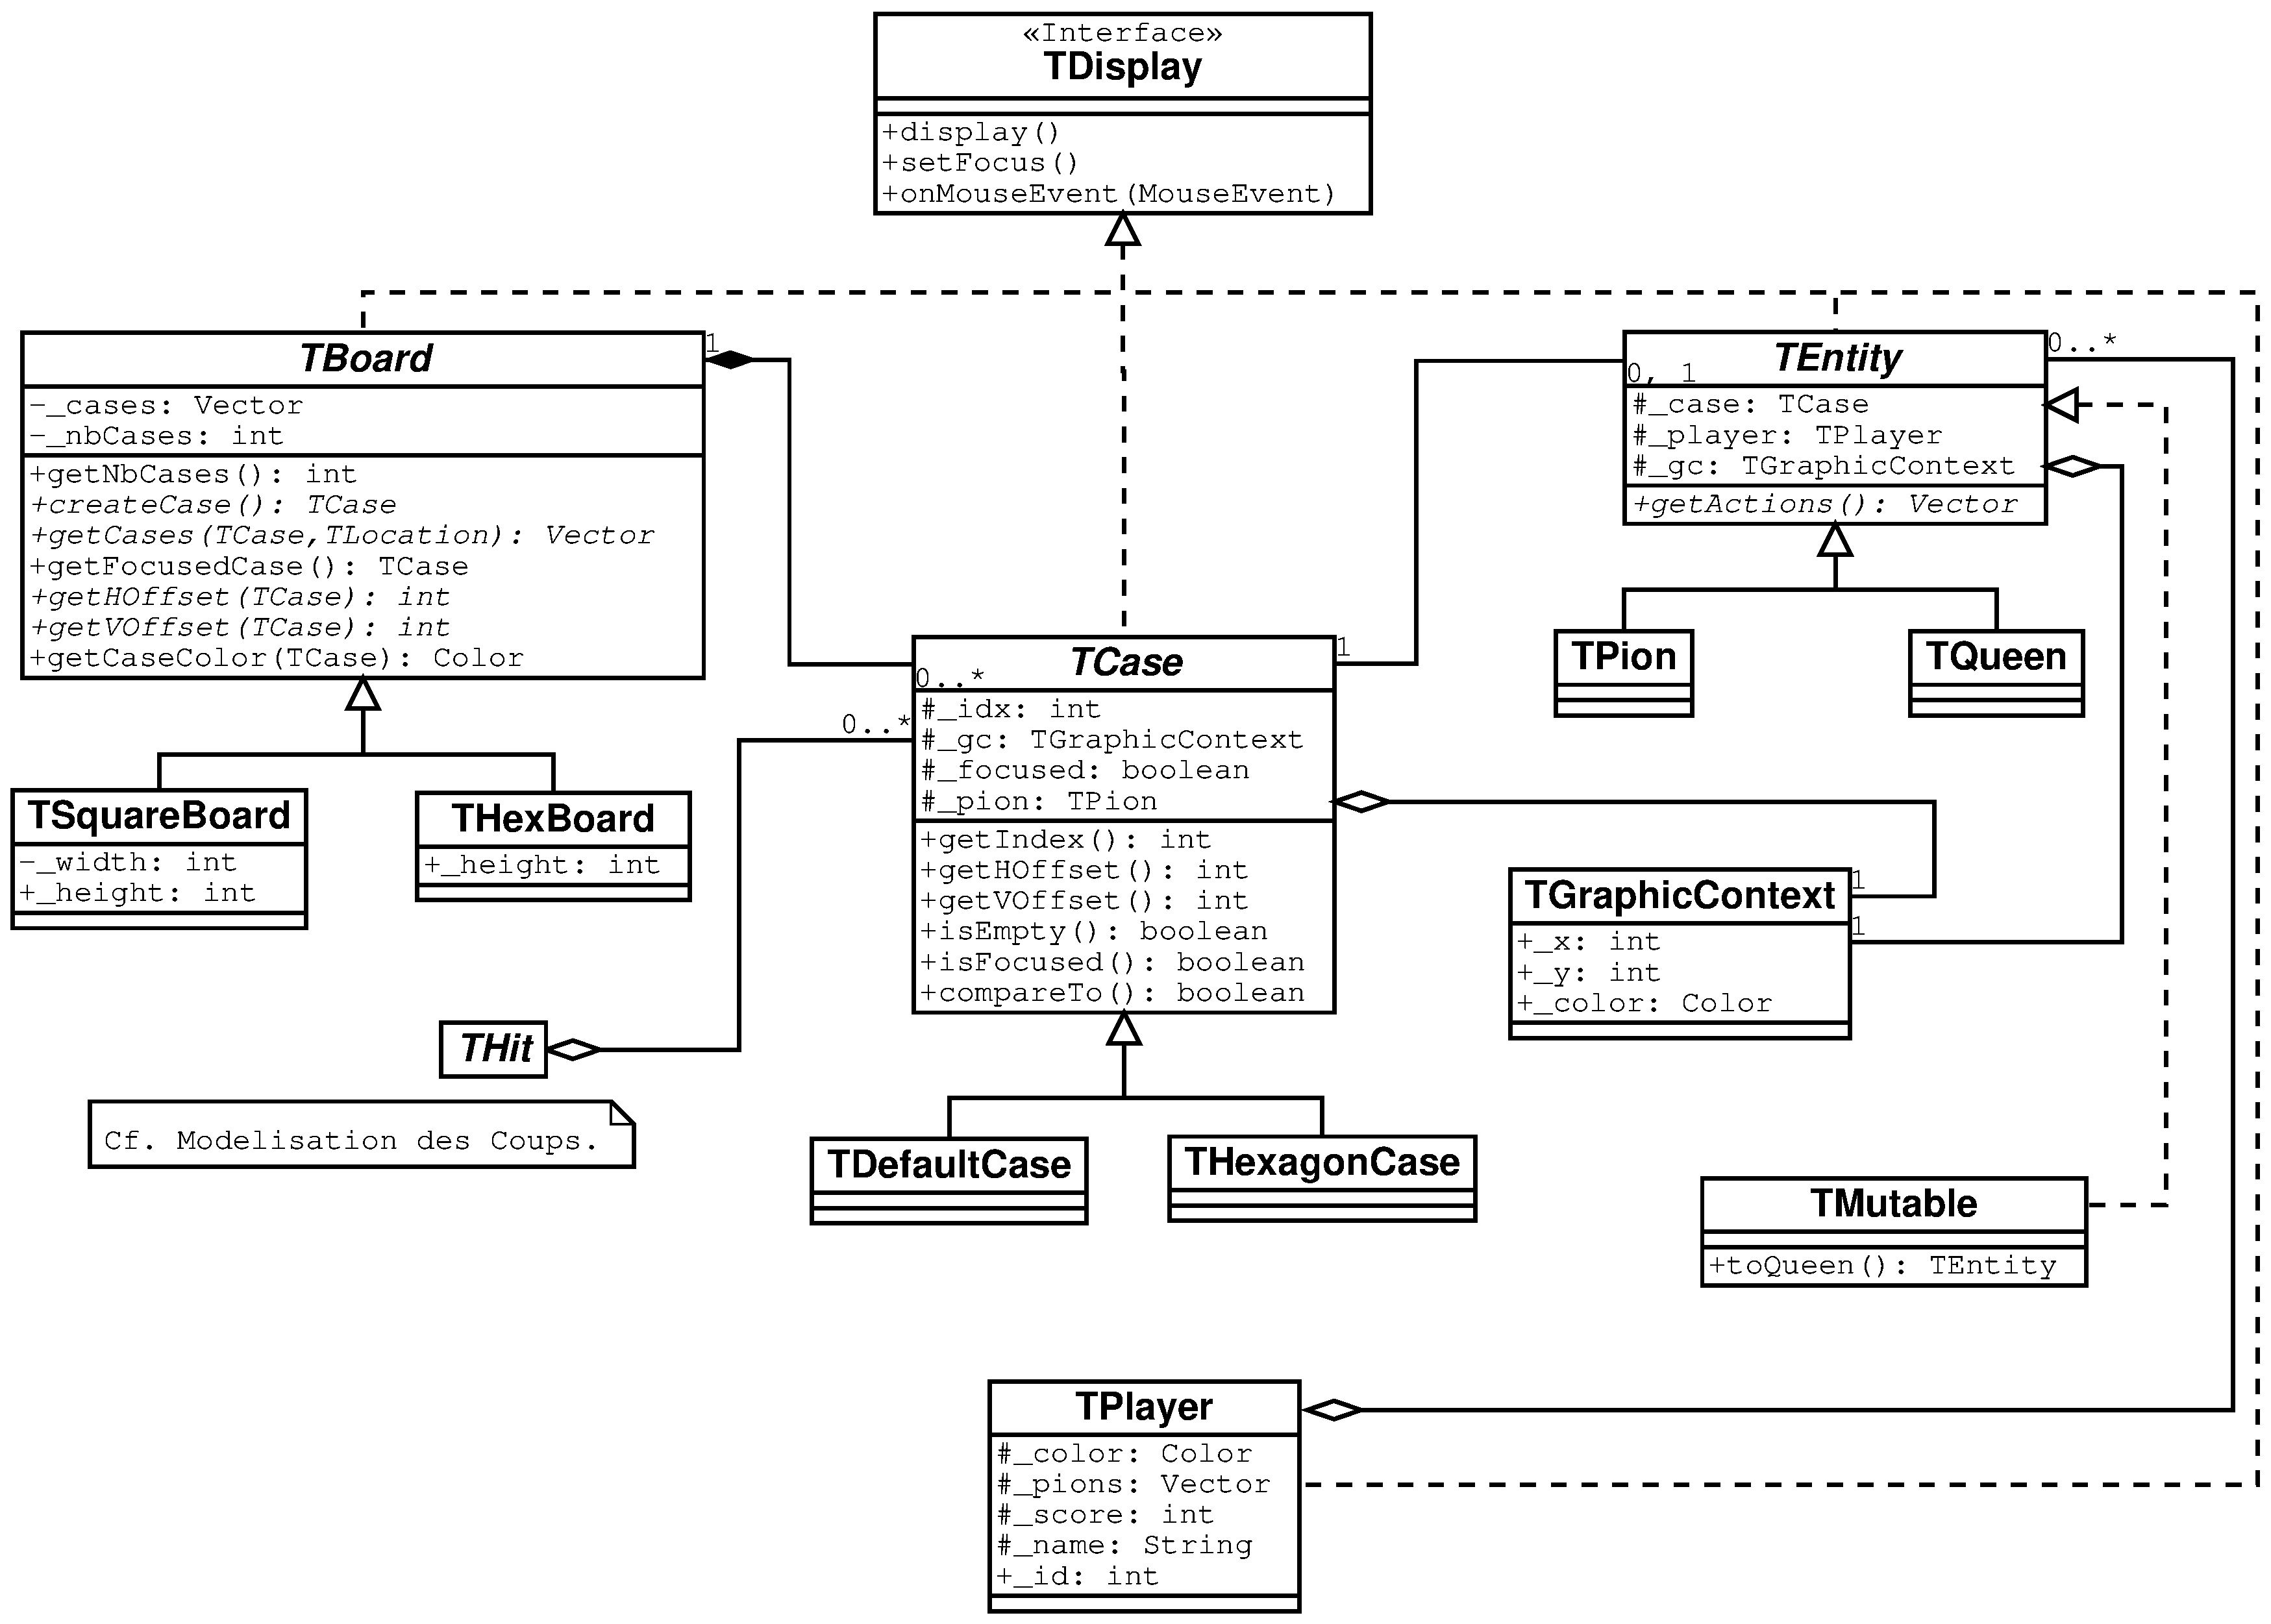
\includegraphics[width=16cm]{MPlateau.eps}
\end{figure}

Modelisation du module Plateau de Jeu

\pagebreak

\begin{figure}[h]
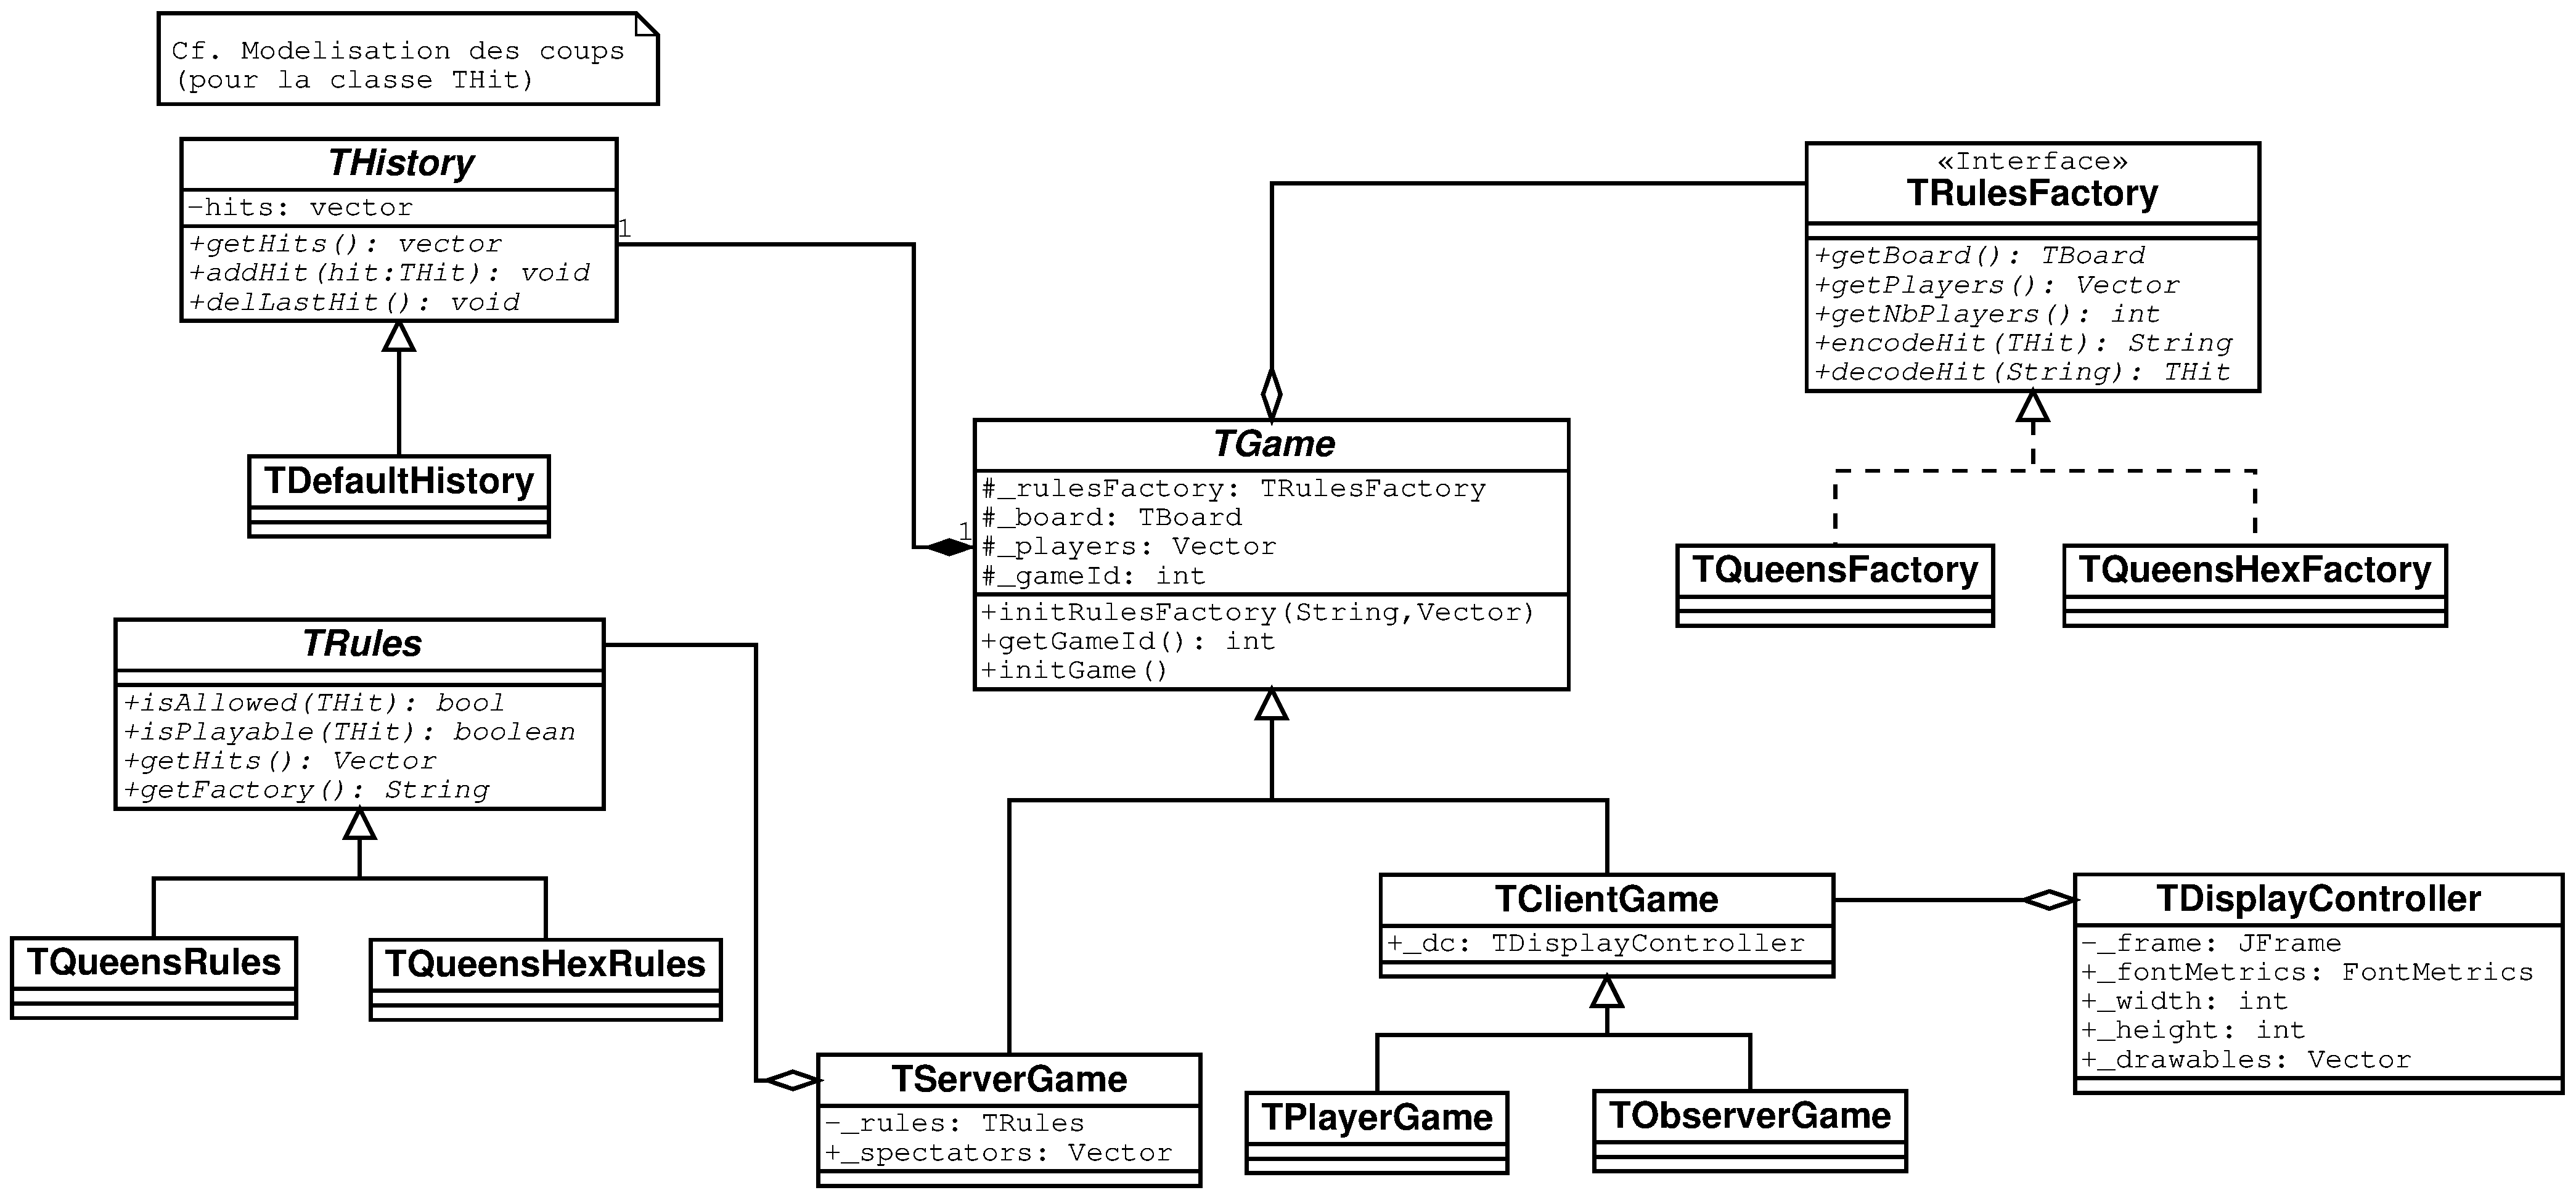
\includegraphics[width=16cm]{MRules.eps}
\end{figure}

Modelisation du module Rules

\pagebreak

\begin{figure}[h]
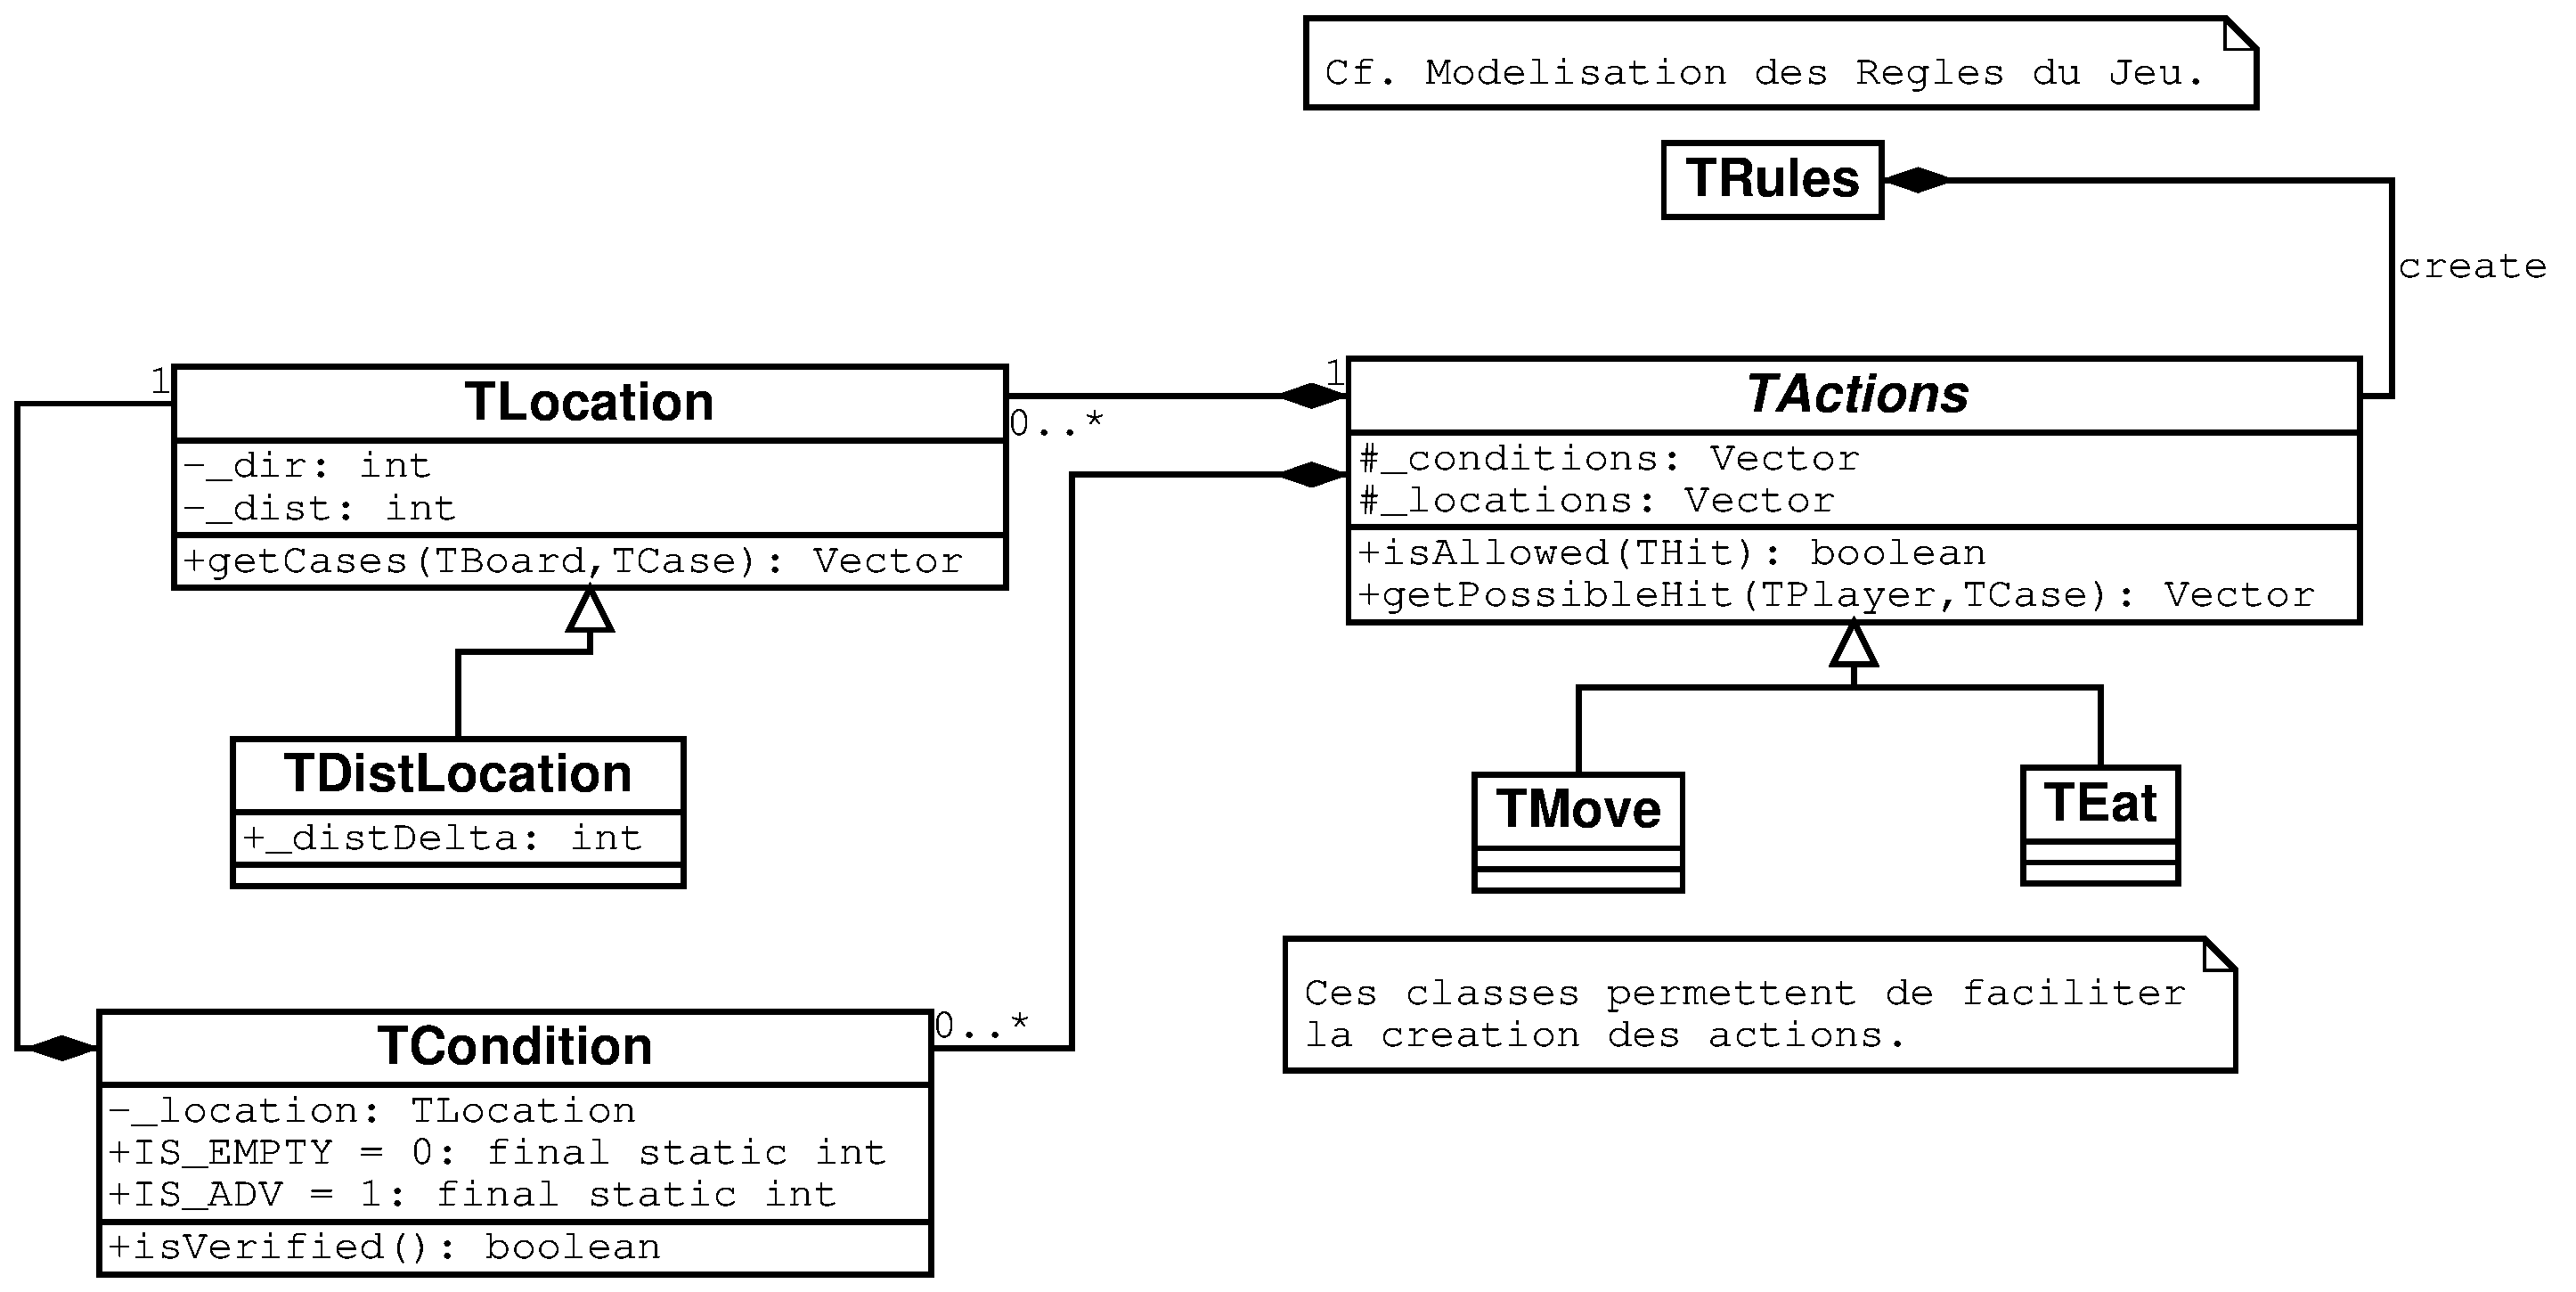
\includegraphics[width=16cm]{MActions.eps}
\end{figure}

Modelisation du module Action

\pagebreak

\begin{figure}[h]
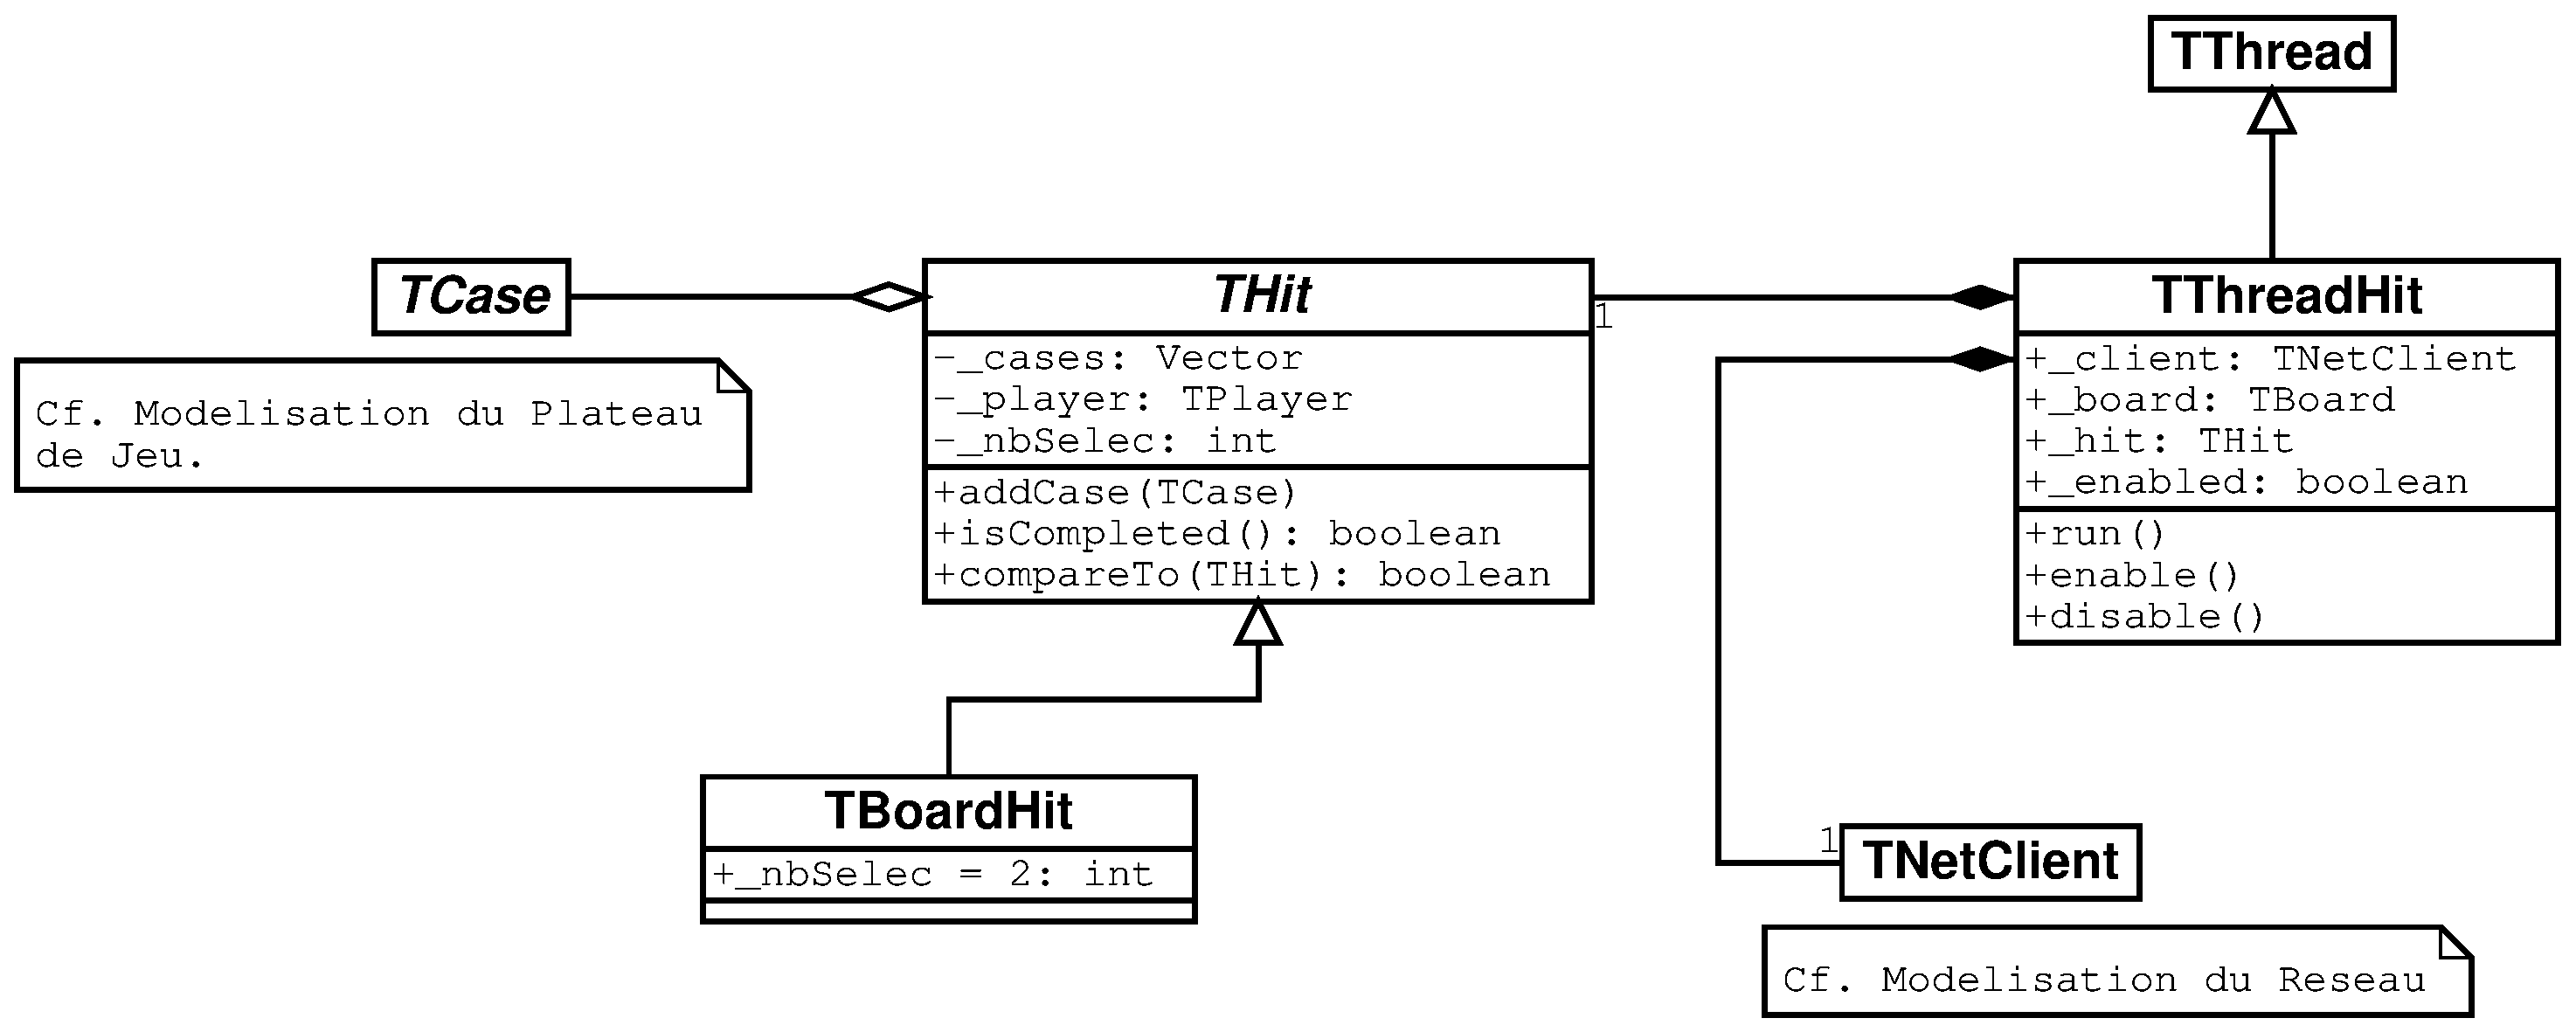
\includegraphics[width=16cm]{MCoups.eps}
\end{figure}

Modelisation du module Coup

\pagebreak

\begin{figure}[h]
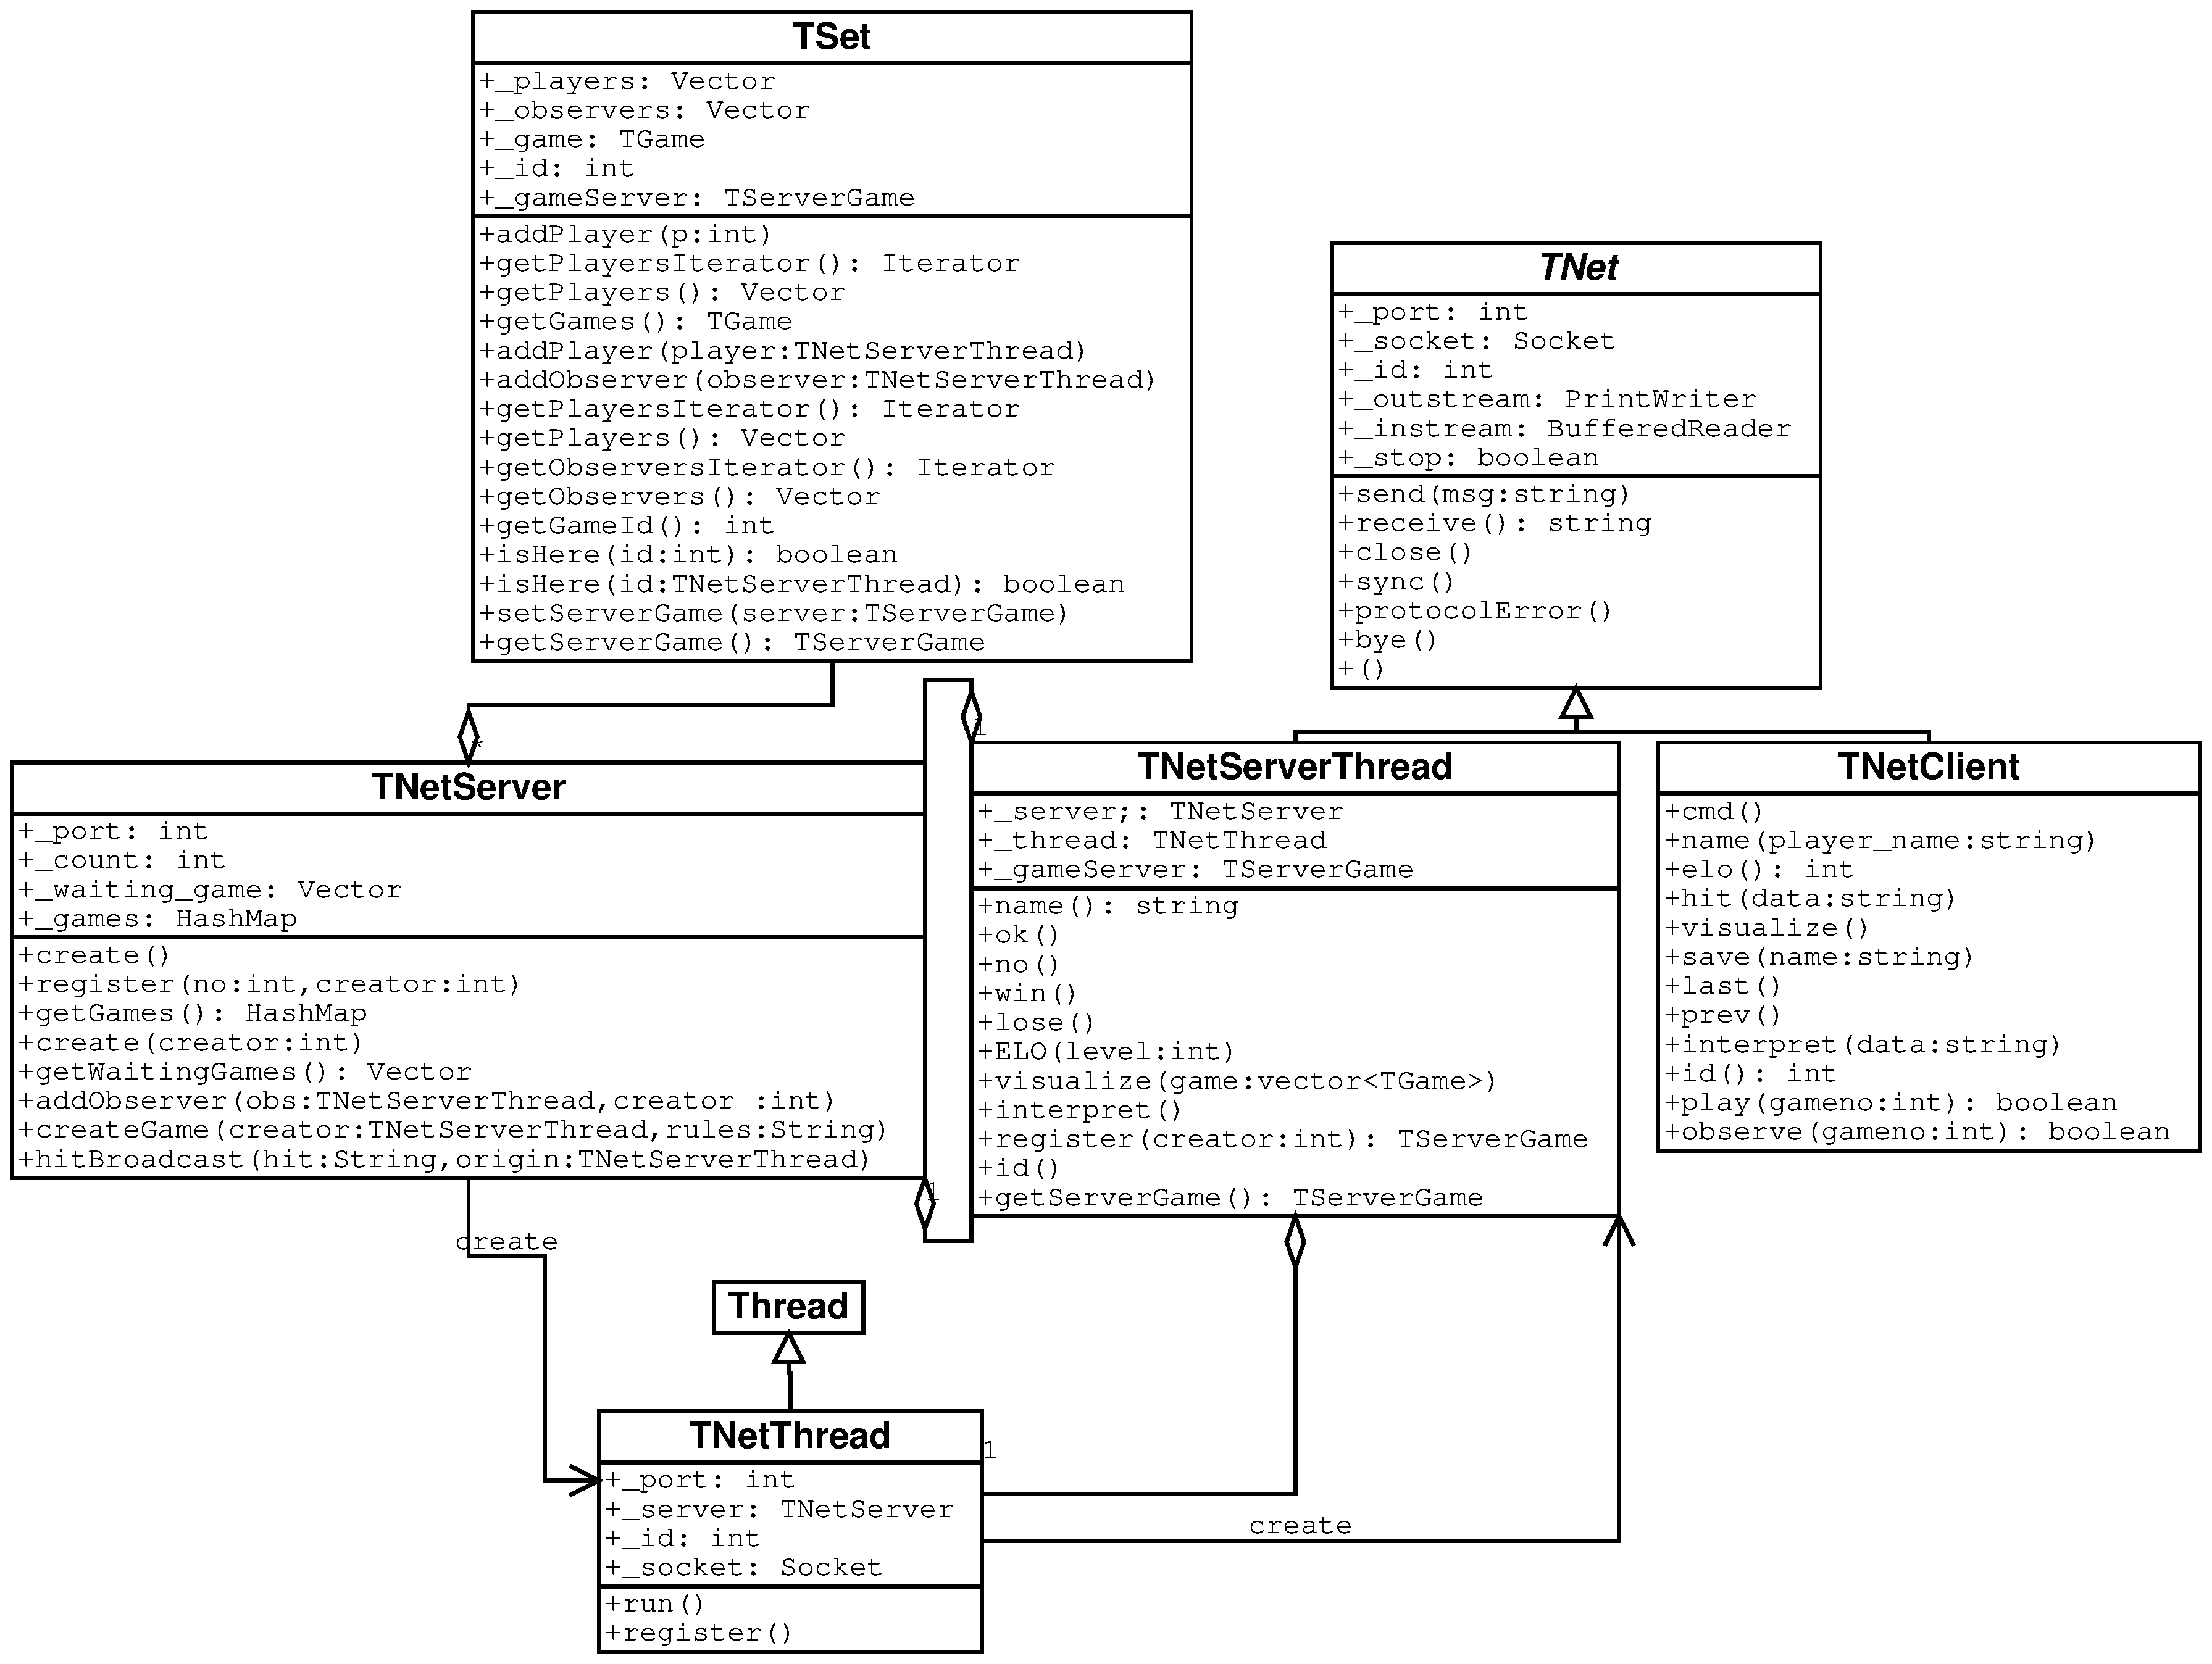
\includegraphics[width=16cm]{MRe.eps}
\end{figure}

Modelisation du module Reseau

\pagebreak

\begin{figure}[h]
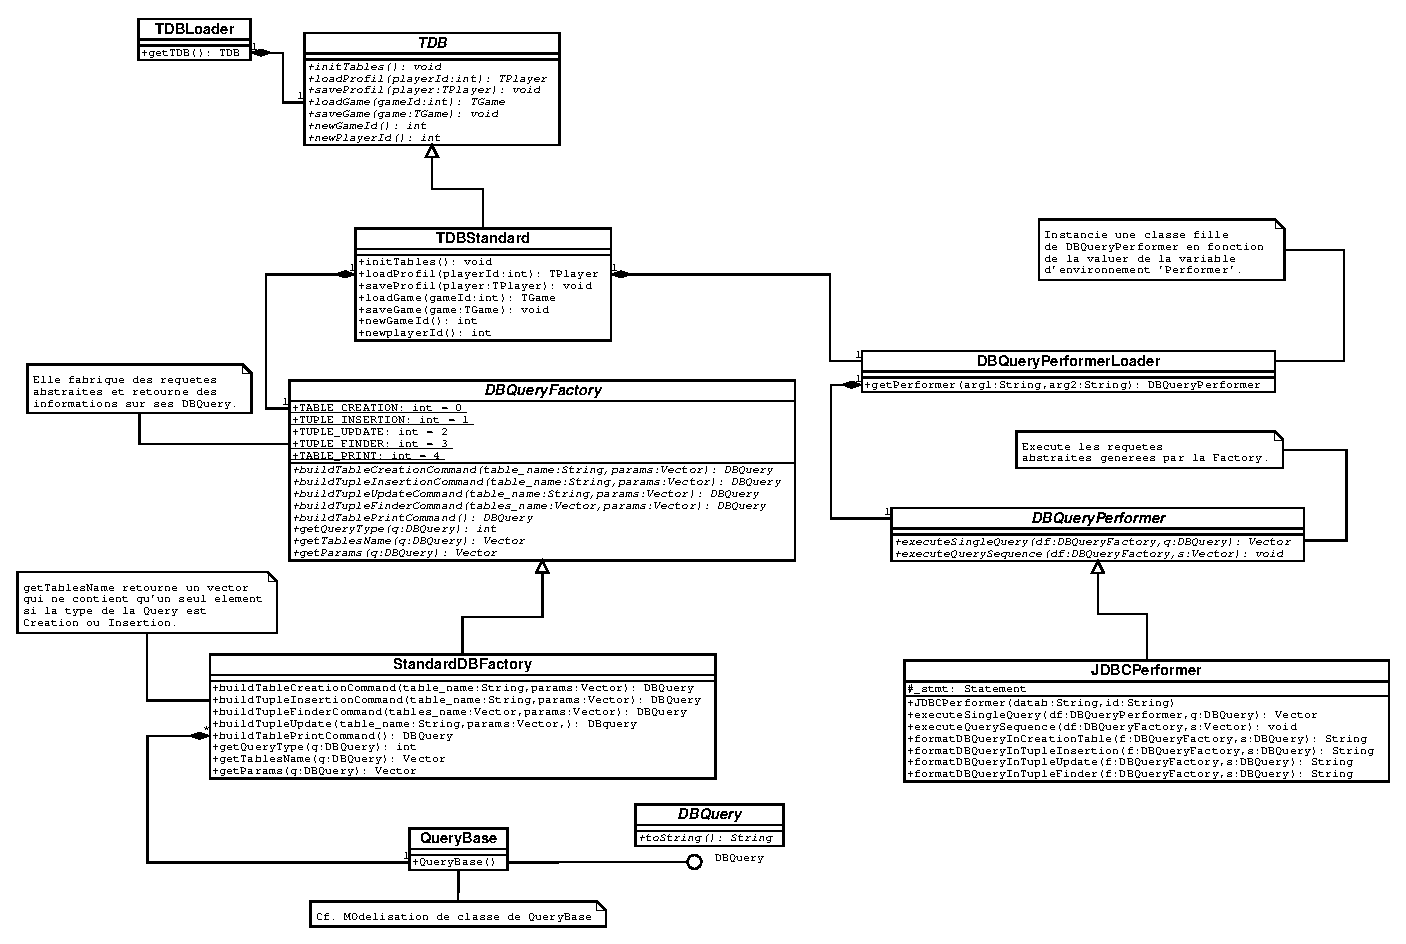
\includegraphics[width=16cm, angle=90]{BDserveur.eps}
\end{figure}

Modelisation du module BD

\pagebreak

\begin{figure}[h]
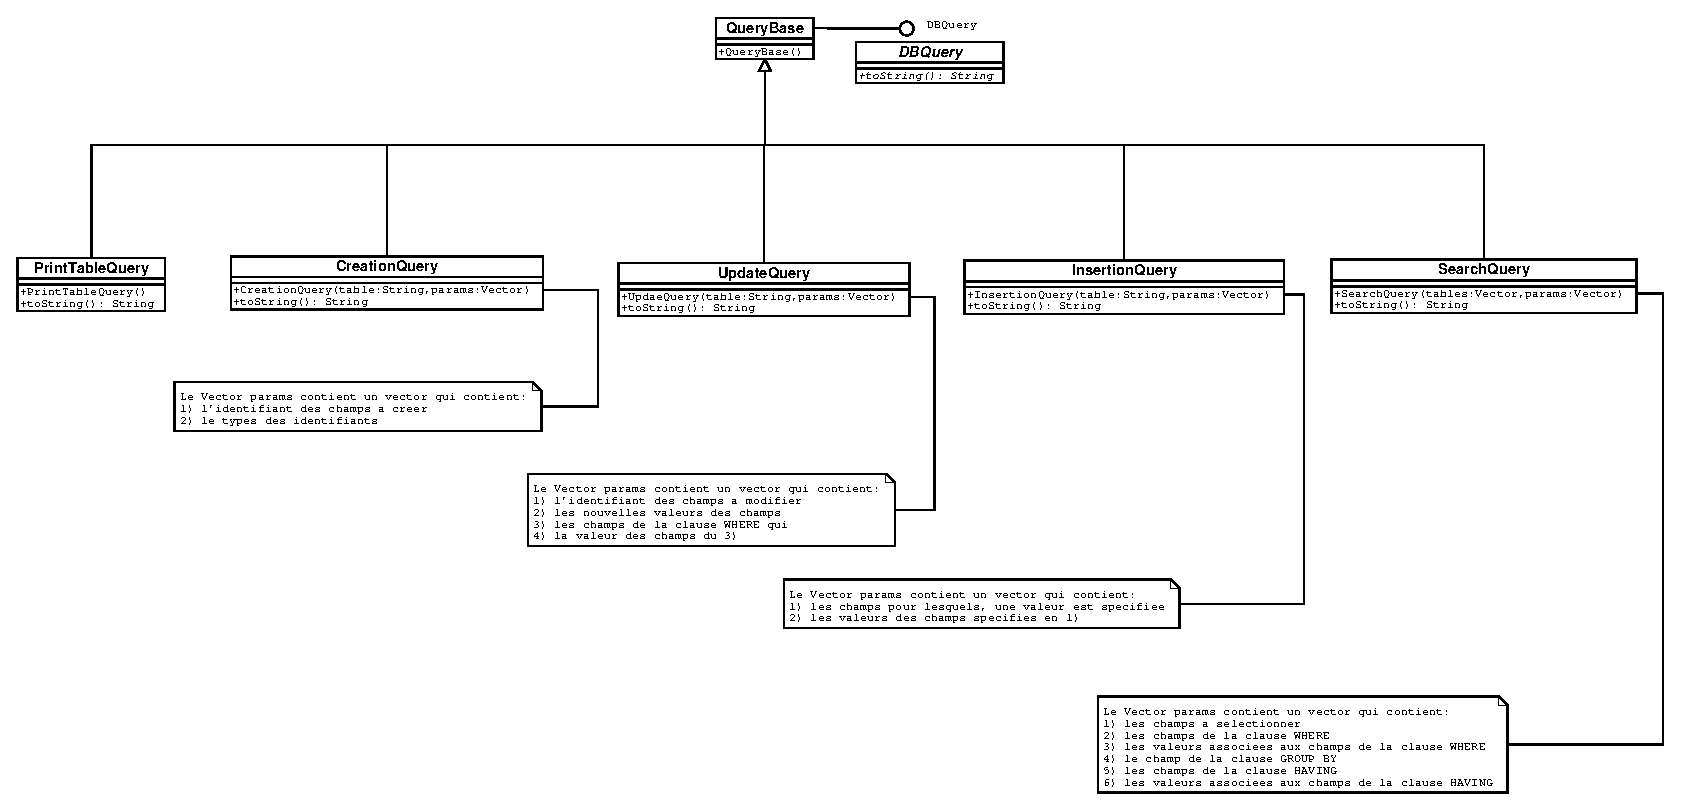
\includegraphics[width=16cm, angle=90]{BDserveurQuery.eps}
\end{figure}

Modelisation des DBquery du module BD

\pagebreak

\begin{figure}[h]
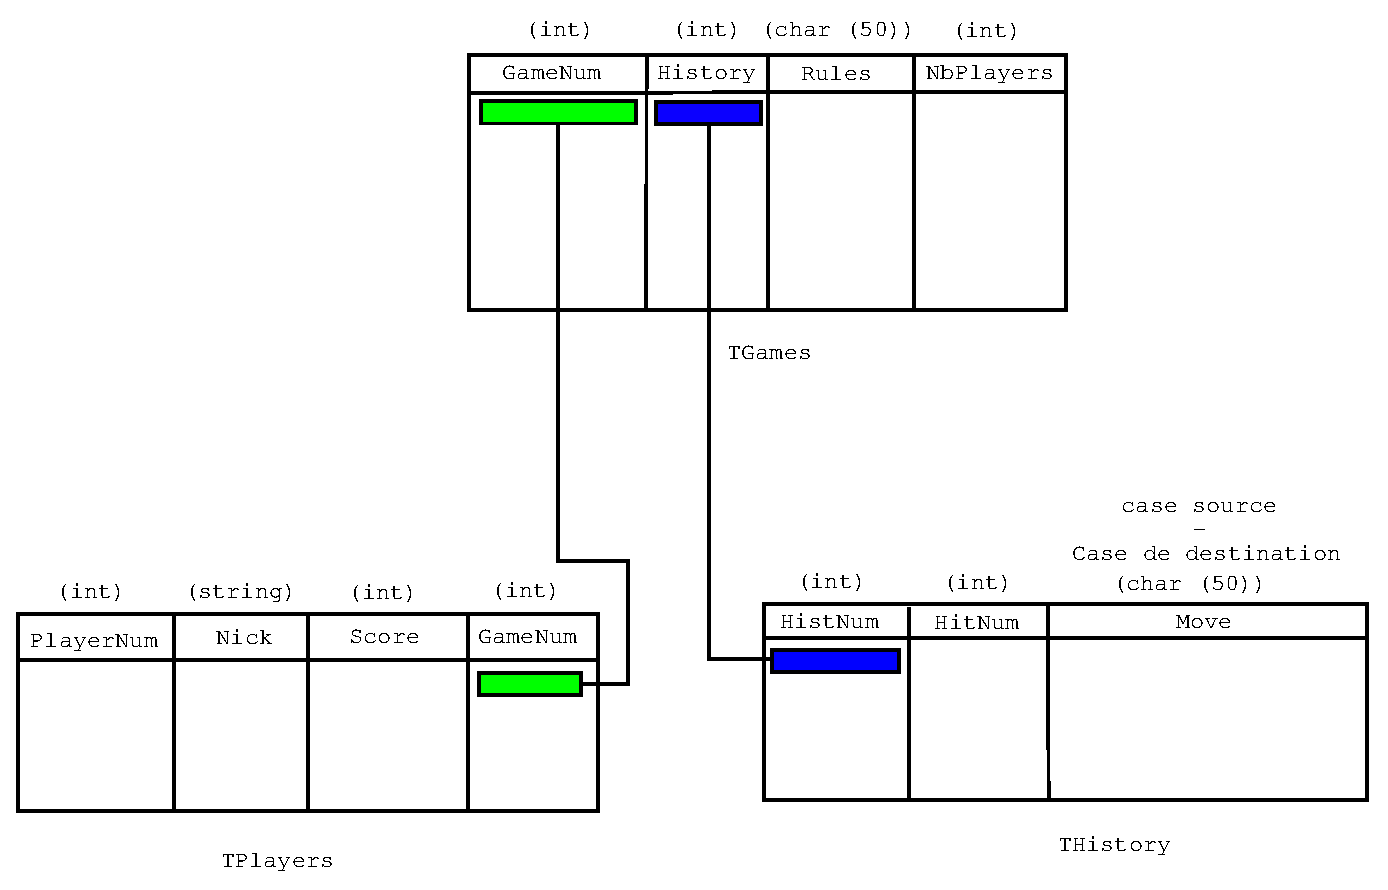
\includegraphics[width=16cm]{BD.eps}
\end{figure}

Une base de donnees type

\end{center}

\pagebreak

\section*{Diagrammes de sequences}
\addcontentsline{toc}{chapter}{Diagrammes de sequences}
\markboth{\uppercase{Diagrammes de sequences}}
{\uppercase{Diagrammes de sequences}}

\begin{center}

\begin{figure}[h]
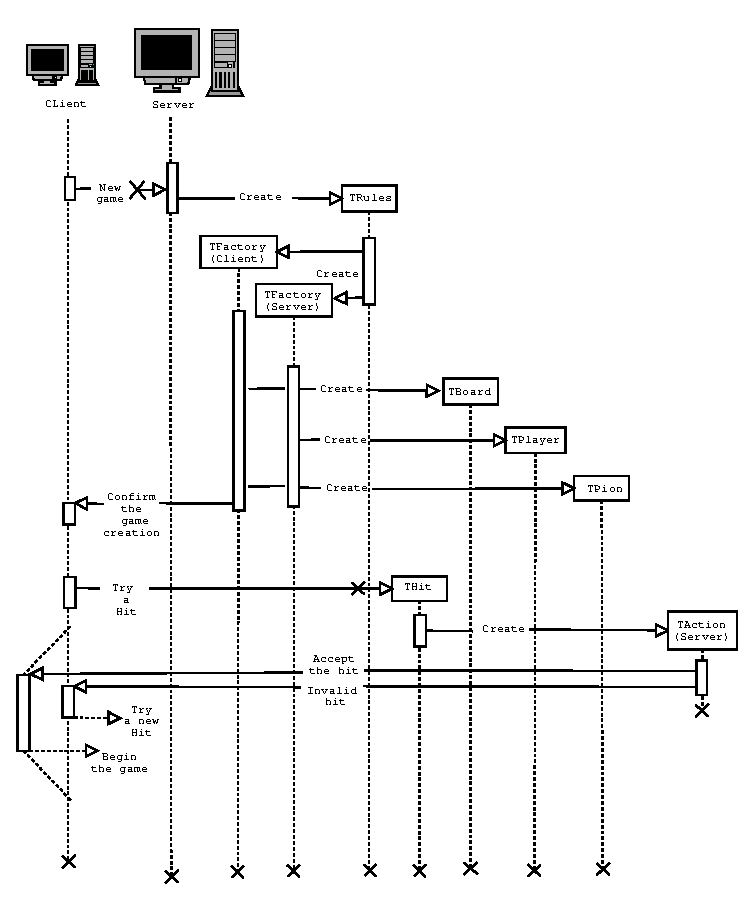
\includegraphics[width=14cm]{DSequenceRules.eps}
\end{figure}

Diagramme de sequence de Rules

\pagebreak

\begin{figure}[h]
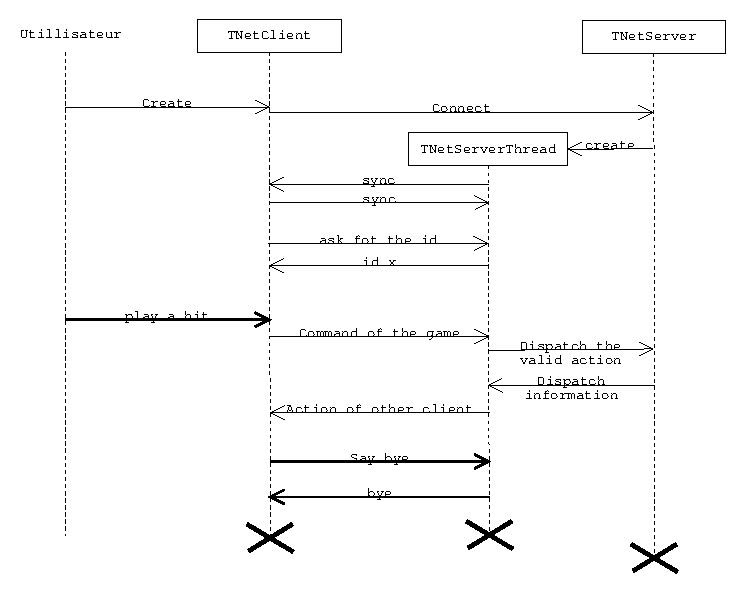
\includegraphics[width=16cm]{DSRe.eps}
\end{figure}

Diagramme de sequence du reseau

\pagebreak

\begin{figure}[h]
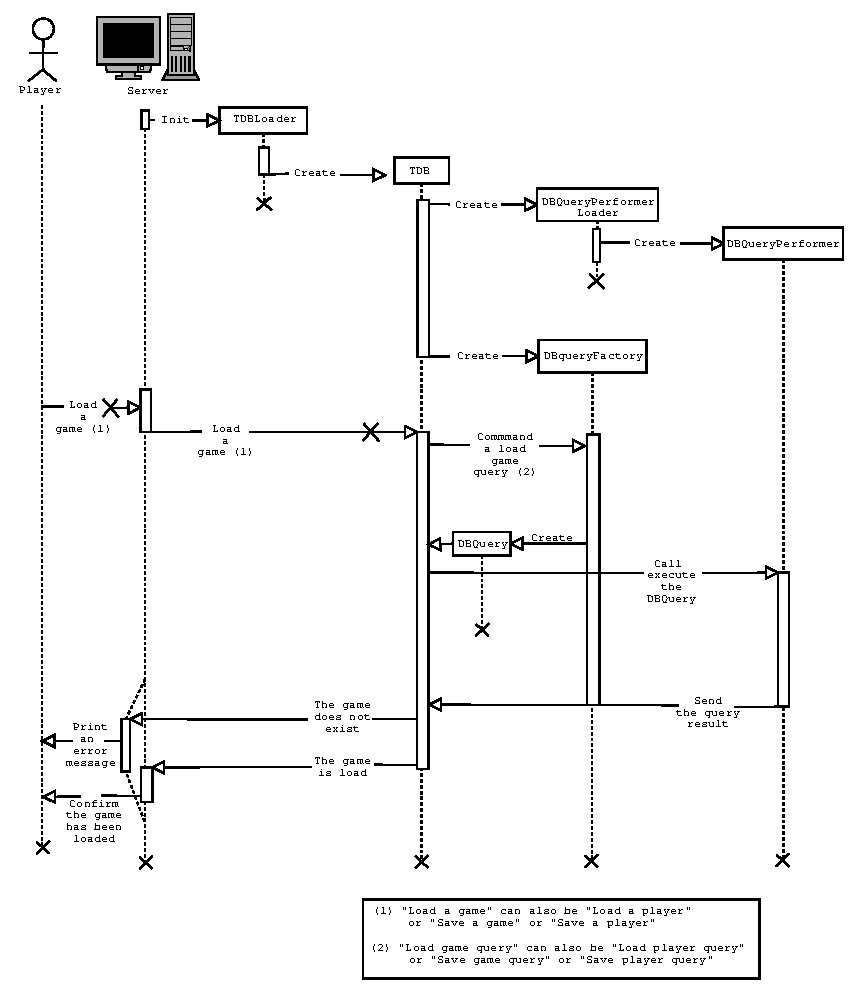
\includegraphics[height=16cm]{DSequenceBD.eps}
\end{figure}

Diagramme de sequence de la Base de Donnees

\end{center}

\pagebreak
	
\section*{Conclusion}
\addcontentsline{toc}{chapter}{Conclusion}
\markboth{\uppercase{Conclusion}}
{\uppercase{Conclusion}}

Nous nous sommes efforc\'es de r\'ealiser une modelisation la plus g\'en\'erique possible.
Le d\'ecoupage du projet en differents modules (r\'eseau, r\`egles du jeu, base de donn\'ees) permet un ajout facile de fonctionnalit\'es.


Malgr\'e les nombreux obstacles qui s'annoncaient: compilation sur les machines Sun, la d\'ependance d'un serveur Mysql rarement \`a notre disposition, nous sommes parvenus \`a realiser un projet extensible :


 - possibilit\'e d'ajout de nouveaux types de plateaux


 - possibilit\'e d'ajout de nouveaux types de pions


 - possibilit\'e d'ajout de nouveaux types d'actions


 - possibilit\'e d'ajout de nouvelles r\`egles de jeu (coup sp\'ecial...)


 - possiblit\'e de r\'eutiliser et d'am\'eliorer le protocol de communication entre les clients et le serveur


 - possibilit\'e d'\'etendre la base de donn\'ees tout en conservant la facilit\'e de g\'en\'eration de requ\`etes.

\end{document}
